\cotefile{22}
\scanpage{2}
C. R. Acad. Sc. Paris, t. 257, p. 2948--2950 (13 novembre 1963). \hfill Groupe 1.

\textsc{Algèbre.} --- \textit{Étude différentielle des anneaux locaux réguliers : applications.}
Note (*) de M. \textsc{Jean-Pierre Jouanolou}, présentée par M. René Garnier.

Le paragraphe 1 donne pour les anneaux locaux usuels (localités, localités analytiques, etc.) une caractérisation différentielle de régularité. Remarquant que, pour ces anneaux, la complétion se fait de façon « séparable », on montre que la réduction et la normalité analytiques en résultent simplement.

1. Les critères différentiels de régularité de Nakai, Suzuki et Mount font \deleted{apparaître}\inserted{appel} en caractéristique $p>0$ \inserted{\unsure{à}}une \deleted{condition}\inserted{\unsure{l'hypothèse}} de réduction analytique (il y a des exemples contraires sinon). L'énoncé suivant permet d'éviter cette condition dans les cas usuels :

\margin{\figure{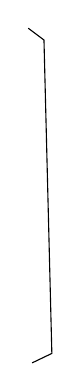
\begin{tikzpicture}[x=1cm,y=1cm]\draw (0.15,0)--(0.4,0.12)--(0.3,4.1)--(0.1,4.25);\end{tikzpicture}}}
\textsc{Proposition 1.} --- \textit{Soient $A$ un anneau local régulier équicaractéristique tel que $D(A)$ soit plat et $\mathfrak{a}$ un idéal de $A$ tel $A/\mathfrak{a}$ soit réduit.}
\margin{\figure{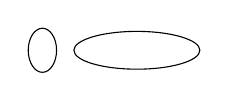
\begin{tikzpicture}\draw (0,0) ellipse (0.18 and 0.28);\draw (1.2,0) ellipse (0.8 and 0.24);\end{tikzpicture}}}

\textit{Les assertions suivantes sont équivalentes :}

\textit{(a) $A/\mathfrak{a}$ est régulier;}

\textit{(b)} $\operatorname{Tor}^{1}_{A/\mathfrak{a}}(A/\mathfrak{m},D(\deleted{A}\inserted{A/\uline{a}}))=0$;

\textit{(c)} $\operatorname{Tor}^{i}_{A/\mathfrak{a}}(A/\mathfrak{m},D(\deleted{A}))=0$ \textit{pour tout $i$ supérieur ou égal à $1$} ($\mathfrak{m}$ \textit{désignant l'idéal maximal de} $A$).

\textit{De plus, si $D(A)$ est libre, (a) équivaut à :}

\textit{(d) $D(A/\mathfrak{a})$ est libre.}

\textsc{Corollaire 1.} --- \textit{Soient $k$ un corps valué complet de caractéristique $p>0$ et tel que $(k:k^p)<+\infty$, $B$ une algèbre de séries convergentes sur $k$ et $A$ un anneau réduit localisé d'un anneau quotient de $B$. Pour que $A$ soit régulier, il faut et il suffit que $D(A)$ soit libre.}

\textsc{Corollaire 2} [Kunz \textsuperscript{(3)}]. --- \textit{Pour qu'une localité \uline{réduite} $A$ soit régulière, il faut et il suffit que son module de différentielles absolu $D(A)$ soit libre.}
\margin{\unsure{contenu dans le critère jacobien} \unsure{---}}

\textsc{Corollaire 3} [Suzuki \textsuperscript{(10)}, Mount \textsuperscript{(5)}]. --- \textit{Soit $A$ un anneau local noethérien analytiquement réduit de caractéristique $p>0$ et tel que le séparé $D'(A)$ \uline{soit de type fini}. Alors, pour que $D'(A)$ soit libre, il faut et il suffit que $A$ soit régulier.}
\margin{\unsure{assez rare !}}

La proposition 1 fournit des critères pour que l'ensemble des points non réguliers du spectre d'un anneau (lieu singulier) soit un fermé, notamment :

\margin{\figure{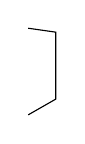
\begin{tikzpicture}\draw (0,1.1)--(0.35,1.05)--(0.35,0.2)--(0,0);\end{tikzpicture}}}
\textsc{Proposition 2.} --- \textit{Si $A$ est un anneau global régulier équicaractéristique tel que $D(A)$ soit libre, le lieu singulier de toute $A$-algèbre affine $B$ est fermé.}
\margin{\unsure{Séries formelles ??}}

En particulier :

\textsc{Proposition 3.} --- \textit{Soit $G$ un schéma en groupes régulier sur un corps parfait. Alors tout schéma de type fini sur $G$ a un lieu singulier fermé.}
\margin{\unsure{Canonique}}

2. Dans tout ce qui suit, $A$ étant un anneau local, nous désignerons par $L_A$ son corps résiduel et par $K_A$ son corps de fractions s'il est intègre.

\mspage{1}

\scanpage{3}
\begin{center}( 2 )\end{center}

Soient $A$ un anneau local noethérien et $\widehat A$ son complété. On a :

\textsc{Lemme.} --- \textit{Le noyau de l'application canonique : $\widehat A\otimes_A D(A)\to D(\widehat A)$ est contenu dans l'intersection : $\displaystyle\bigcap_{M\in\sigma}\left(\widehat A\otimes_A M\right)$, où $\sigma$ désigne l'ensemble des sous-modules $M$ de $D(A)$ tels que $F=D(A)/M$ soit un $A$-module de type fini.}

De ce lemme on déduit que si $D(A)$ est semi-fini au sens de Suzuki \textsuperscript{(10)}, c'est-à-dire somme directe d'un module libre et d'un module de type fini, la suite canonique
\diagram{\begin{tikzcd}[ampersand replacement=\&]
0\arrow[r]\&\widehat A\otimes_A D(A)\arrow[r]\&(\widehat A)\arrow[r]\&D_A(\widehat A)\arrow[r]\&0
\end{tikzcd}}
est exacte.

Cela entraîne notamment :

\textsc{Proposition 4.} --- \textit{Si $A$ est une localité analytiquement \uline{intègre}, $K_{\widehat A}$ est séparable sur $K_A$.}

De même (\textit{cf.} cor. 1 de la prop. 1), si $A$ est un anneau de séries convergentes sur un corps valué complet de caractéristique $p>0$ et tel que $(k:k^p)<+\infty$, $K_{\widehat A}$ est séparable sur $K_A$. Ceci permet de combler ce qui nous paraît être une lacune dans la démonstration donnée par Lang \textsuperscript{(4)} du résultat suivant :

\textsc{Proposition 5.} --- \textit{Si $A=k\{T\}$ est l'anneau des séries convergentes sur un corps $k$ valué complet et algébriquement clos, $K_A$ est quasialgébriquement clos $(C^1)$.}

Un cas particulier de la proposition 4, classique, est que $K((X_1,X_2,\ldots,X_n))$ est séparable sur $K(X_1,\ldots,X_n)$ pour tout corps $K$. Il implique, en tenant compte du théorème de structure de Cohen :

\textsc{Proposition 6.} --- \textit{Soit $A$ un anneau local régulier contenant un corps $k$ tel que $L_A$ soit séparable sur $k$. Alors $K_A$ est aussi séparable sur $k$.}
\margin{\figure{\begin{tikzpicture}[y=1cm]\draw (0,5.8)--(0.2,5.85)--(0,0.05)--(-0.2,0);\node[right] at (0.4,3.4) {\unsure{connu}};\end{tikzpicture}}}

3. \textsc{Critère de réduction analytique.} --- La comparaison de la proposition 1 et des énoncés de Suzuki et Mount suggère l'existence d'un critère de réduction analytique sous-jacent; nous nous proposons de voir dans ce paragraphe comment les conclusions du paragraphe 2 permettent d'en obtenir un. Notons tout d'abord le lemme suivant qui peut être considéré comme classique :

\textsc{Lemme.} --- \textit{Soit $A$ un anneau local noethérien analytiquement intègre et tel que $K_{\widehat A}$ soit séparable sur $K_A$. Si $B$ est un anneau local intègre de la forme $B=C_{\mathfrak p}$, où $C$ est une $A$-algèbre \uline{finie} et $\mathfrak p$ un idéal premier de $C$ tel que $\mathfrak p\cap A=\mathfrak M$ ($\mathfrak M$ idéal maximal de $A$), $B$ est analytiquement réduit.}
\margin{\unsure{faux si on ne suppose pas} $A\to B$ \unsure{injectif} ??}

On en déduit :

\textsc{Théorème.} --- \textit{Soit $A$ un anneau local régulier vérifiant l'une ou l'autre des conditions suivantes :}

$(h_1)$ \textit{$K_A$ est de caractéristique $0$;}

$(h_2)$ \figure{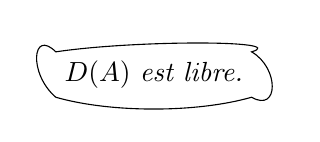
\begin{tikzpicture}[baseline=(t.base)]\node[inner sep=3pt] (t) {$D(A)$ \textit{est libre.}};\draw (t.south west) .. controls +(-0.35,0.3) and +(-0.3,0.3) .. (t.north west) .. controls +(1,0.15) and +(0.5,0.15) .. (t.north east) .. controls +(0.35,-0.2) and +(0.35,-0.2) .. (t.south east) .. controls +(-0.7,-0.2) and +(0.7,-0.2) .. (t.south west);\end{tikzpicture}}

\mspage{2}

\scanpage{4}
\begin{center}( 3 )\end{center}

\textit{Alors toute $A$-algèbre intègre qui est localisée d'une $A$-algèbre finie (i. e. $A$-module de type fini) $C$\inserted{$C\supset A$ !!!} est analytiquement réduite.}

(Pour appliquer le lemme, on remarque que $h_1$ et $h_2$ sont stables par localisation.)
\margin{\figure{\begin{tikzpicture}[x=1cm,y=1cm]\draw (0.25,0.3) .. controls (-0.5,-0.7) and (-0.6,0.4) .. (0.05,0.65);\draw (-0.1,-0.1) .. controls (1,-0.25) and (3,0) .. (4,0.1);\node[right] at (4.15,0.1) {faux};\end{tikzpicture}}}

De l'existence de lemmes de normalisation [pour les séries convergentes, \textit{voir} \textsuperscript{(5)} par exemple], on déduit :

\textsc{Corollaire 1} (Chevalley). --- \textit{Toute localité intègre est analytiquement réduite.}

\textsc{Corollaire 2.} --- \textit{Soient $k$ un corps d'exposant caractéristique $p$ tel que $(k:k^p)<+\infty$, $B$ une algèbre de séries convergentes sur $k$ et $A$ un anneau intègre localisé d'un anneau quotient de $B$. Alors $A$ est analytiquement réduit.}

Dans le même ordre d'idées, notons la :

\textsc{Proposition 7.} --- \textit{Soit $A$ un anneau local noethérien analytiquement intègre et tel que $K_{\widehat A}$ soit séparable sur $K_A$. Alors la fermeture intégrale de $A$ dans toute extension finie $L$ de $K_A$ est un $A$-module de type fini.}
\margin{\figure{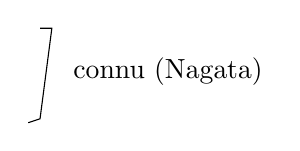
\begin{tikzpicture}\draw (0,1.2)--(0.15,1.2)--(0,0.05)--(-0.15,0);\node[right] at (0.3,0.65) {\unsure{connu} (Nagata)};\end{tikzpicture}}}

La proposition 7 s'applique aux localités, aux localités \uline{analytiques} et aux algèbres de Hopf régulières sur un corps parfait.
\margin{?}

D'après le lemme 2 (p. 314, chap. 8, § 13) de \textsuperscript{(11)}, on voit alors par exemple qu'une localité analytique vérifiant les conditions du corollaire 2 et normale est analytiquement normale.
\margin{\figure{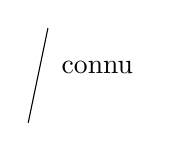
\begin{tikzpicture}\draw (0,0)--(0.25,1.2);\node[right] at (0.3,0.7) {\unsure{connu}};\end{tikzpicture}}}

(*) Séance du 4 novembre 1963.

\textsuperscript{(1)} \textsc{Berger} et \textsc{Kunz}, \textit{Math., Z.}, \textbf{77}, 1961, p. 314-338.

\textsuperscript{(2)} \textsc{Godement}, \textit{Séminaire Cartan-Chevalley}, 1955-1956, exp. 17, 18, 19.

\textsuperscript{(3)} \textsc{Kunz}, \textit{Math. Z.}, \textbf{76}, 1961, p. 56-74.

\textsuperscript{(4)} \textsc{Lang}, \textit{Ann. Math.}, \textbf{55}, 1952, p. 373-390.

\textsuperscript{(5)} \textsc{Mount}, \textit{Proc. Amer. Math. Soc.} juin 1963.

\textsuperscript{(6)} \textsc{Nagata}, \textit{Locals rings}, Inters., Tracts n° 13, 1962.

\textsuperscript{(7)} \textsc{Nagata}, \textit{On the closedness of singular loci}, Publ. I. H. E. S., n° 2, 1959.

\textsuperscript{(8)} \textsc{Nakai}, \textit{J. Math. Soc. Japan}, \textbf{13}, 1961, p. 63-84.

\textsuperscript{(9)} \textsc{Nakai} et \textsc{Suzuki}, \textit{J. Sc. Hiroshima Univ.}, série A, \textbf{23}, 1960, p. 459-476.

\textsuperscript{(10)} \textsc{Suzuki}, \textit{J. Math. Kyoto Univ.}, \textbf{2}, 1963, p. 157-182.

\textsuperscript{(11)} \textsc{Zariski} et \textsc{Samuel}, \textit{Commutative Algebra}, Van Nostrand.

\hfill (7, \textit{rue Chernoviz, Paris}, 16\textsuperscript{e}).

\mspage{3}

\scanpage{5}
\hrule
165.056. --- Imp. \textsc{Gauthier-Villars} \& C\textsuperscript{ie}, 55, Quai des Grands-Augustins, Paris (6\textsuperscript{e}).

\begin{center}Imprimé en France.\end{center}

\mspage{\unsure{4}}

\scanpage{6}
\textit{C. R. Acad. Sc.}, t. 256, p. 842-844. \hfill Séance du 21 janvier 1963. \hfill Groupe 1

\textsc{Algèbre.} --- \textit{Sur les modules de différentielles.}

Note (*) de M. \textsc{Jean-Pierre Jouanolou}, présentée par M. René Garnier.

Application des modules de différentielles aux algèbres quasi-séparables et aux anneaux locaux réguliers.

$A$ et $B$ désignent dans toute cette Note deux anneaux commutatifs et unitaires, $u:A\to B$ un monomorphisme unitaire et $D_A(B)$ le $B$-module des différentielles de l'algèbre ainsi définie. Le passage de cette situation « globale » à la situation « locale » se fait en imposant à $A$, $B$, $u$ d'être locaux; l'idéal maximal de $A$ (resp. $B$) sera en ce cas noté $\mathfrak m$ (resp. $\mathfrak n$) et son corps résiduel $L_a$ (resp. $L_b$); par ailleurs, le rang de $\mathfrak m$ est $\operatorname{rg}\mathfrak m=\dim_{L_a}(\mathfrak m/\mathfrak m^2)$, et de même pour $\mathfrak n$. Rappelons qu'étant donnée une extension de corps : $K\to L$, la dimension du $L$-espace vectoriel $D_K(L)$ représente en caractéristique $0$ (resp. $p>0$) le degré de transcendance de $L$ par rapport à $K$ (resp. le nombre d'éléments d'une $p$-base de $L$ par rapport à $K$) : on la notera $\{L:K\}$ dans tous les cas.

Nous nous proposons d'étudier d'abord les cas où $D_A(B)$ est nul, puis ceux où il est libre (en liaison avec la régularité des anneaux locaux), le tout grâce aux deux suites exactes établies dans le cadre local par Berger et Kunz \textsuperscript{(1)} :

\diagram{\begin{tikzcd}[ampersand replacement=\&]
0\arrow[r]\&\dfrac{\mathfrak n}{\mathfrak n^2+\mathfrak m B}\arrow[r]\&L_b\otimes_B D_A(B)\arrow[r]\&D_{L_a}(L_b)\arrow[r]\&0,
\end{tikzcd}}

\diagram{\begin{tikzcd}[ampersand replacement=\&]
0\arrow[r]\&\dfrac{\mathfrak n}{\mathfrak n^2+(\mathfrak n\cap A[B^p])B}\arrow[r]\&L_b\otimes_B D_A(B)\arrow[r]\&D_{L_a}(L_b)\arrow[r]\&0.
\end{tikzcd}}

La première est vraie si $L_b$ est séparable sur $L_a$, la deuxième, sinon : alors $p>0$ désigne la caractéristique des corps résiduels.

1. \textsc{Structure des algèbres quasi-séparables.} --- Une $A$-algèbre $B$ est dite \uline{quasi-séparable} lorsque $D_A(B)=0$. Il s'agit là d'une propriété locale, en ce sens que $B$ est quasi-séparable si pour tout idéal maximal $\mathfrak n$ de $B$, $B_{\mathfrak n}$ est quasi-séparable sur $A_{\mathfrak m}$ ($\mathfrak m=\mathfrak n\cap A$), et seulement en ce cas.
\margin{\uline{\unsure{non ramifiée}}}

\textit{Localement :}

(i) Si $L_b$ est séparable sur $L_a$ (en particulier en caractéristique $0$) : lorsque $B$ est quasi-séparable,
\[
(\mathrm R)\quad \mathfrak n=\mathfrak n^2+\mathfrak mB,
\]
et $L_b$ est algébrique (resp. relativement parfait \textsuperscript{(2)}) sur $L_a$ en caractéristique $0$ (resp. $p>0$) la réciproque étant vraie si l'on suppose, en outre, que $D_A(B)$ est de type fini. Notons que si $B$ est noethérien, ou plus généralement si $\mathfrak n$ est de type fini, la relation (R) s'écrit
\[
\mathfrak n=\mathfrak mB,
\]
ce qui exprime que $B$ n'est pas ramifié sur $A$.
\margin{!?}

\mspage{5}

\scanpage{7}
\begin{center}( 2 )\end{center}

(ii) En caractéristique $p>0$ (pour les corps résiduels) : si $B$ est quasi-séparable, $L_b$ est relativement parfait \textsuperscript{(2)} sur $L_a$ et
\[
(\mathrm S)\quad \mathfrak n=(\mathfrak n\cap A[B^p])B+\mathfrak n^2,
\]
la réciproque étant vraie si l'on suppose en outre $D_A(B)$ de type fini. Si $B$ est noethérien, (S) se simplifie encore.

\textit{Globalement :}

(i) Soit $A$ un anneau noethérien quasi-séparable sur un corps $K$ :

--- en caractéristique $0$, $A$ est composé direct d'une famille finie d'extensions algébriques de $K$;

--- en caractéristique $p>0$, si pour tout idéal maximal de $A$ le corps résiduel est une extension séparable (resp. de type fini) de $K$, $A$ est composé direct d'une famille finie d'extensions séparables et quasi-séparables (resp. algébriques séparables) de $K$.

(ii) Soit $A$ une algèbre quasi-séparable sur un corps $K$ :

--- en caractéristique $0$, tout idéal premier de $A$ est maximal et tous les corps résiduels des localisés de $A$ sont des extensions algébriques de $K$;

--- en caractéristique $p>0$, si pour tout idéal premier $\unsure{\mathfrak q|\mathfrak g}$ de $A$ le corps $A_{\unsure{\mathfrak q}}/\unsure{\mathfrak q}A_{\unsure{\mathfrak q}}$ est de type fini sur $K$, alors tout idéal premier de $A$ est maximal et tous les corps résiduels sont des extensions algébriques séparables de $K$;

--- Sous l'une ou l'autre de ces hypothèses, le quotient de $A$ par sa nilracine est un anneau absolument plat \textsuperscript{(3)}.

2. \textsc{Différentielles et anneaux locaux réguliers.} --- On se place dans le cadre local, en supposant même $A$ et $B$ intègres, de corps des fractions $K_a$ et $K_b$, et les cardinaux $\{L_b:L_a\}$, $\{K_b:K_a\}$, $\operatorname{rg}\mathfrak n$ finis.

\textsc{Théorème.} --- \textit{Si $D_A(B)$ est de type fini (en particulier si $B$ est de type fini sur $A$) il y a équivalence entre :}

(i) \textit{$D_A(B)$ est libre;}

(ii) \textit{a. Dans le cas où $L_b$ est séparable sur $L_a$ :}
\[
\dim_{L_b}\frac{\mathfrak n}{\mathfrak n^2+\mathfrak mB}=\{K_b:K_a\}-\{L_b:L_a\};
\]

\textit{b. Sinon, $p>0$ désignant la caractéristique de $L_b$ et $L_a$ :}
\[
\dim_{L_b}\frac{\mathfrak n}{\mathfrak n^2+(\mathfrak n\cap A[B^p])B}=\{K_b:K_a\}-\{L_b:L_a\}.
\]

Notons que l'hypothèse « $D_A(B)$ de type fini » entraîne que les cardinaux $\{K_b:K_a\}$ et $\{L_b:L_a\}$ sont finis. De plus, l'égalité (ii) $a$ s'écrit :

--- Si $A$ est un corps : $\operatorname{rang}\mathfrak n=\{K_b:A\}-\{L_b:A\}$,

--- Si $B$ est non ramifié sur $A$ : $\{K_b\mid K_a\}=\{L_b\mid L_a\}$.

\mspage{6}

\scanpage{8}
\begin{center}( 3 )\end{center}

\textsc{Corollaire.} --- \textit{Si $A$ est une localité sur le corps $K$, telle que $K_a$ et $L_a$ soient séparables sur $K$, il y a équivalence entre :}

(i) \textit{$D_K(A)$ est libre;}

(ii) $A$ est régulier.

\textsc{Proposition 1.} --- \textit{Si $A$ domine un corps $K$, tel que $D_K(A)$ soit libre et de rang fini, si $K_b$ (resp. $L_a$) est séparable sur $K_a$ (resp. $L_b$) et si}
\[
\operatorname{rg}\mathfrak n-\operatorname{rg}\mathfrak m=\{K_b:K_a\}-\{L_b:L_a\},
\]
\textit{$D_A(B)$ est un $B$-module de dimension homologique finie $\leqq1$.}

\textsc{Corollaire.} --- \textit{Si $A$ est un anneau local régulier contenant un corps $K$, tel que le couple $(K,A)$ jouisse des propriétés énoncées dans le corollaire ci-dessus, $D_A(B)$ est de dimension homologique $\leqq1$ sous les hypothèses de la proposition 1.}

\textsc{Proposition 2.} --- \textit{Soit $A$ un anneau local noethérien contenant un corps $K$ tel que $\{L_a:K\}$ soit fini et que $L_a$ soit séparable sur $K$. Si $D_K(A)$ est libre, de rang $\dim A+\{L_a:K\}$, $A$ est local régulier.}

Notons, pour conclure, que dans de nombreuses questions (\textit{cf.} géométrie formelle) il vaut mieux séparer $D_A(B)$ en considérant
\[
D'_A(B)=\frac{D_A(B)}{\displaystyle\bigcap_{n\geqq0}\mathfrak n^n D_A(B)};
\]
la proposition 2 est encore vraie, lorsqu'on y substitue $D'_K(A)$ à $D_K(A)$.

(*) Séance du 14 janvier 1963.

\textsuperscript{(1)} \textsc{Berger} et \textsc{Kunz}, \textit{Math. Z.}, \textbf{77}, 1961, p. 314-338.

\textsuperscript{(2)} \textsc{Bourbaki}, \textit{Algèbre}, chap. V, § 8, ex. 1.

\textsuperscript{(3)} \textsc{Bourbaki}, \textit{Algèbre comm.}, chap. I, § 2, ex. 17.

\textsuperscript{(4)} \textsc{Godement}, \textit{Séminaire Cartan-Chevalley}, 1955-1956, exposés 17 et 18.

\textsuperscript{(5)} \textsc{Nakai}, \textit{J. Math. Soc. Japan}, 1961.

\textsuperscript{(6)} \textsc{Nakai} et \textsc{Suzuki}, \textit{J. Sc. Hiroshima Univ.}, série A, \textbf{24}, n° 3, décembre 1960.

\hfill (\textit{École Normale Supérieure, 45, rue d'Ulm, Paris}, 5\textsuperscript{e}.)

\mspage{7}

\scanpage{9}
\hrule
163.228. --- Imp. \textsc{Gauthier-Villars} \& C\textsuperscript{ie}, 55, Quai des Grands-Augustins, Paris (6\textsuperscript{e}).

\begin{center}Imprimé en France.\end{center}

\mspage{8}

\scanpage{10}
\mspage{24}
\margin{$/^{\circ}[\,]$ inutile, \unsure{résulte du} \deleted{\unsure{fait}} que $IB$ (\unsure{resp.} $IC$) top. nilpotent.}

\uline{contenant $IB$ resp. $IC$}\inserted{]}\unsure{,} enfin on suppose $IB$ et $IC$ fermés (condition automatiquement vérifiée si $B,C$ sont noethériens). \unsure{Soient}\deleted{\unsure{u}} $B_0=B/IB$,\deleted{et} $C_0=C/IC$, $u:\inserted{B\to C}$ un homomorphisme continu de $A$-algèbres, $u_i:B_i\to C_i$ l'homomorphisme \deleted{induit} déduit par passage au quotient (j'ai oublié d'introduire un système fondamental d'idéaux ouverts $I_i\subset I_0\inserted{=I}$ dans $A$, et les $B_i$ et $C_i$ en conséquence\inserted{enfin ce sont tous les $I_iB$ et $I_iC$ qui doivent être fermés}). Conditions équivalentes:

(i\inserted{bis}) $u$ est \deleted{un isomorphisme} bijectif, et \figure{\begin{tikzpicture}[baseline=(t.base)]\node[draw,ellipse,inner sep=4pt] (t) {$u_0$ est un homéomorphisme.};\draw[->] (t.east)--++(0,0.8);\end{tikzpicture}}

(i\deleted{bis}) $u$ est un isomorphisme d'algèbres topologiques
\margin{\figure{\begin{tikzpicture}\draw[->] (0,0)..controls (-0.5,0.5) and (-0.5,0.85)..(0.8,1.1);\end{tikzpicture}}}

(ii) Pour tout $i$, $u_i:B_i\to C_i$ est bijectif, \figure{\begin{tikzpicture}[baseline=(t.base)]\node[draw,ellipse,inner sep=4pt] (t) {$u_0$ est un homéomorphisme};\draw[->] (t.east)--++(0,0.8);\end{tikzpicture}}

(ii bis) pour tout $i$, munissant $B_i$ et $C_i$ des filtrations $I$-adiques, l'homomorphisme $\operatorname{gr}_I(B_i)\to\operatorname{gr}_I(C_i)$ induit par $u\deleted{\unsure{e}}$ est bijectif, \figure{\begin{tikzpicture}[baseline=(t.base)]\node[draw,ellipse,inner sep=4pt,align=left] (t) {$u_0$ un\\homéomorphisme.};\draw[->] (t.east)--++(0,0.9);\end{tikzpicture}}

\margin{On \unsure{suppose} dès le début}

Enfin, lorsque les $\deleted{B}\inserted{C}_i$ sont plats sur les $A_i$, \unsure{les} conditions équivalent également à

(iii) $u_0:B_0\to C_0$ est un \deleted{isomorphisme} \figure{\begin{tikzpicture}[baseline=(t.base)]\node[draw,ellipse,inner sep=4pt] (t) {homéomorphisme.};\draw[->] (t.east)--++(0,0.8);\end{tikzpicture}}

L'équivalence de (i) et (i bis) résulte trivialement du fait que les topologies de $B,C$ sont \deleted{adiques} définies par les puissances d'idéaux contenant $IB$ resp. $IC$. \deleted{\unsure{Celle de}} Evidemment $(\mathrm i\inserted{bis})\Rightarrow(\mathrm {ii})$, pour $(\mathrm {ii})\Rightarrow(\mathrm i\inserted{bis})$ on note que les applications canoniques $B\to\underset{\inserted{\leftarrow}}{\lim}B_i$ et $C\to\underset{\inserted{\leftarrow}}{\lim}C_i$ sont bijectives grâce au fait que les $I_iB$ et $I_iC$ sont fermés (cf rectification à $0_{\inserted{7.2.4.}}$). L'équivalence de (ii) et (ii bis), \deleted{\unsure{qu}} mise pour mémoire, provient du fait que ($I=I_0$ étant un idéal de définition, donc nilpotent dans les $A_i$) les filtrations mises sur $B,C$ sont finies. Enfin, reste à prouver que lorsque \deleted{\unsure{B est p}} $\deleted{B}\inserted{C}_i$ est plat sur $A_i$, alors $u_0$ bijectif implique $u_i$ bijectif ou si on veut $\operatorname{gr}(u)$ bijectif, ce qui est immédiat et sauf erreur figure déjà en lemme quelque part au Chap III (j'espère, avec la généralité qui convient, et bien entendu modulé ...).

\margin{Cf diagramme}
\diagram{\begin{tikzcd}[ampersand replacement=\&]
\operatorname{gr}B\arrow[r,"\mathrm{surj}"] \& \operatorname{gr}C\\
B_0\otimes\operatorname{gr}\unsure{A_i|A'}\arrow[u,"\mathrm{surj}"]\arrow[r,Rightarrow,"\mathrm{bij}"'] \& C_0\otimes\operatorname{gr}\unsure{A_i|A'}\arrow[u,"\mathrm{bij}"']
\end{tikzcd}}

\mspage{9}

\scanpage{11}
\mspage{25}

Enfin, il nous sera commode d'avoir un critère permettant de déduire
de la propriété P une propriété de platitude. Nous utiliserons :

\uline{Lemme} \inserted{4.}3. Soient $A$ un anneau, $(P_i)_{i\in I}$ une famille de $A$-modules,
\inserted{$P$ leur produit} $M$ un $A$-module de présentation finie. Alors l'homomorphisme canonique
\[
M\otimes P\longrightarrow\prod M\otimes P_i
\]
est un isomorphisme.

En effet, écrivant $M$ comme comme un conoyau d'un homomorphisme
de modules libres \inserted{de type fini} $L'\longrightarrow L$, et notant que le foncteur produit est exact
donc exact à gauche, on est ramené au cas où $M=A^n$, $n$ entier $>0$, où
c'est trivial.

\uline{Corollaire} \inserted{4.}4. Supposons $A$ tel que tout module de type fini sur $A$ soit
de présentation finie, par exemple $A$ noethérien. Alors tout produit de
$A$-modules plats est un $A$-module plat.

En effet, il suffit de montrer que $P\otimes$ transforme un monomorphisme
$M\longrightarrow N$ en un monomorphisme, quand $M$ et $N$ sont de type fini; le lemme 3 donne
alors immédiatement le résultat voulu.

\uline{Corollaire} \inserted{4.}5. Supposons que $A$ satisfasse \deleted{\unsure{les hypothèses}}
\inserted{\unsure{la condition}} de \inserted{4.}4. \inserted{par exemple $A$ noethérien} Soit
$P$ un $A$-module \deleted{topologique} isomorphe à \unsure{une} limite projective
\deleted{\unsure{``stricte'' ``dénombr''}}
\deleted{de $A$-modules projectifs de type fini (``stricte'' = par un système projectif strict),
``dénombrable'' par un système proje}
\deleted{Alors $P$ est un $A$}
d'un système projectif strict, \deleted{de $A$}
admettant un système cofinal dénombrable, de $A$-modules projectifs. Alors
$P$ est un $A$-module plat.

En effet, on voit facilement que sous les conditions dites, $P$ est
isomorphe à un produit de $A$-modules projectifs, donc plats, d'où le résultat.

\mspage{10}

\scanpage{12}
\mspage{26}

\uline{Théorème} \inserted{4.}6. Soient $A$ un anneau préadmissible muni d'un idéal de
définition $I=I_0$ et d'un système fondamental $(I_i)$ d'idéaux de définition
$I_0$, $B$ une $A$-algèbre topologique. On suppose\deleted{\unsure{x}} les $A_i=A/I_iA$ noethériens,
et de plus les conditions suivantes sur $B$:

\deleted{\unsure{a) Les} $\unsure{A_i=A/I_i}$ \unsure{noethériens}}

\unsure{a)} Les module\deleted{s} topologique\deleted{s}
\deleted{$\unsure{B_i=B/I_iB}$} \inserted{$B$ sur $A$}
\deleted{\unsure{sont}} satisf\deleted{ont}\inserted{ait} la condition P.

\inserted{b) $B_0$ est formellement simple sur $A_0$}

\deleted{b)}\inserted{c)} $B$ est adique \deleted{pour un idéal contenant $IB$}

\inserted{d)} Les idéaux $I_iB$ dans $B$ sont fermés (\deleted{inutile}\inserted{automatiquement vérifié} si $B$ est noethérien).

Sous ces conditions, on a ce qui suit\deleted{\unsure{x}}:

(i) $B$ est formellement simple sur $A$.

(ii) Soit $C$ une $A$-algèbre topologique satisfaisant à \unsure{c)} et d)
(mais pas nécessairement à a) ), et soit $u_0:B_0\xrightarrow{\sim}C_0$ un isomorphisme
d'algèbres topologiques. Alors il existe un $A$-homomorphisme continu
$u:B\longrightarrow C$ se réduisant suivant $u_0$ (en vertu de (i) et de 1.7.). Ce
dernier étant choisi, les conditions suivantes sont équivalentes: \deleted{\unsure{1°}}

\deleted{\unsure{a)}}\inserted{1)} $B$ est formellement simple sur $A$.

2) \deleted{$B$ est} $B$ satisfait la condition a) ci-dessus, i.e. \deleted{est} satisfait
la condition P.

3) Les $B_i$ sont plats sur $A_i$.

4) L'homomorphisme $u:B\longrightarrow C$ est un isomorphisme\deleted{\unsure{,}} de $A$-algèbres top.

\inserted{5) $\unsure{C}$ est \unsure{isom.} à $B$ comme $A$-algèbre top.}

Démonstration. L'assertion (i) résulte déjà de a)\inserted{et b)}, grâce à 3.1.
Prouvons donc (ii). En vertu de (i) déjà prouvé, on a $2)\Longrightarrow1)$, et
Evidemment $4)\Longrightarrow2)$, d'ailleurs $2)\Longrightarrow3)$ en vertu de 3.5., grâce au
fait que les $A_i$ sont noethériens. Reste à prouver $1)\Longrightarrow4)$ et $3)\Longrightarrow4)$.

Supposons 1) vérifié, alors en vertu de 1.7. $u_0^{-1}:C_0\longrightarrow B_0$
se prolonge en un homomorphisme d'algèbres top $v:C\longrightarrow B$ (grâce aux
hypothèses \unsure{c)} et d) ). On a déjà noté que les $B_i$ sont plats sur les
$A_i$. Le lemme \inserted{4.}2. (i) et (iii) (où on échange les rôles de $B,C$)

\mspage{11}

\scanpage{13}
\mspage{27}

garantit alors que $v$ est un isomorphisme d'algèbres topologiques (grâce
à \unsure{c)} et d) pour $B$ et $C$). Donc \deleted{les} on a 2), \deleted{et}
\inserted{donc on a 3). Or} le même argument en
sens inverse montre que \deleted{$\unsure{u:C\longrightarrow B}$ est alors un isomorphisme d'alg top, i.e.
qu'on a 4)} \inserted{3) implique 4). -- Enfin $4)\Longrightarrow5)$ et $5)\Longrightarrow2)$.}
On peut certainement améliorer la rédaction de la démonstration, évitant certaines redites.

Pour simplifier, nous nous restreindrons par la suite à des hypothèses
noethériennes (permettant de nous débarrasser en particulier de la désagréable hypothèse d) sur $B$).

\uline{Définition} \inserted{4.}7. Soit $A\longrightarrow B$ un homomorphisme continu d'anneaux noethériens
préadiques. On dit que $B$ est une \uline{algèbre} (topologique) \uline{de Cohen} sur $A$
si \inserted{a)} $B$ est séparé et complet, i.e. \inserted{est} un anneau adique,
\deleted{\unsure{pourvu}} \inserted{b)} s'il satisfait à la condition P, et si enfin \inserted{c)} $B$ est formellement
\deleted{\unsure{plat}} \inserted{simple} sur $A$, \deleted{\unsure{ou}}
\inserted{(ou encore, $I$ étant un idéal de définition de $A$, $B_0=B/IB$ est formel\textsuperscript{\unsure{t}} simple sur $A_0=A/IA$)}

On notera qu'en vertu de 3.1., si $I$ est un idéal de définition de $A$,
la dernière condition équivaut à la condition que $B/IB$ est formellement
simple sur $A/IA$. D'ailleurs, on peut interpréter \inserted{4.}6. de la façon
suivante (et il est \deleted{peut-être} plus raisonnable de reléguer \inserted{4.}6. en lemme,
et de réserver le corollaire en théorème):

\uline{Corollaire} \inserted{4.}8. Soient $A$ un anneau \deleted{préadique} noethérien, $I$ un idéal de $A$,
munissons $A$ de la topologie $I$-préadique, posons $A_0=A/IA$, et soit $B_0$ une
$A_0$-algèbre topologique. \deleted{Si il}\inserted{Supposons qu'il} existe une algèbre de Cohen $B$ sur $A$ telle
que $B/IB$ soit isomorphe à $B_0$ comme $A_0$-algèbre topologique,
\inserted{(ce qui implique $B_0$ \deleted{\unsure{formellement simple}}\inserted{\unsure{anneau de Cohen}} sur $A_0$).}
alors $B$ est unique à \inserted{un} isomorphisme près
\deleted{(induisant l'isomorphisme donné sur} (compatible avec les isomorphismes donnés des algèbres
\deleted{réduites} réduites mod $I$ avec $B_0$). De plus, si $B$ est une $A$-algèbre topologique adique telle que $B/IB$
soit isomorphisme à $B_0$ comme $A_0$-algèbre topologique, alors les conditions
suivantes sur $B$ sont équivalentes: \inserted{a)} $B$ est une $A$-algèbre de Cohen

\mspage{12}

\scanpage{14}
\mspage{28}

1) $B$ est formellement simple sur $A$

2) $B$ satisfait la condition P \quad 3) $B$ est plat sur $A$ \quad 3 bis) Pour tout
entier $n\geq0$, $B_n=B/I^{n+1}B$ est plat sur $A_n=A/I^{n+1}$. \deleted{4)}

Il reste seulement à montrer l'équivalence de 3) et 3 bis), qui est
contenue en effet (moyennant les hypothèses noethériennes faites) dans
la platitude supérieure.

\deleted{Le résultat précédent} Il conviendrait de noter aussi \inserted{dès après 3.7.} que ``algèbre de
Cohen'' est une notion stable par extension de la base via produits tensoriels complétés: c'est une trivialité.

Le résultat \inserted{4.}8. montre l'intérêt qu'il y a, $A,I$ et $B_0$ étant donnés,
de disposer d'un \uline{théorème d'existence} pour une algèbre de Cohen $B$ sur $A$
se réduisant suivant $B_0$. On notera que la construction habituelle de
proche en proche nous ramène \deleted{au cas où $A$ est discr}(remplaçant $A$ par des $A_i$
et $I$ par des puissances) au cas où $I$ est de carré nul, (donc où $A$ est
discret). On obtient alors un problème de nature essentiellement infinitésimale,
dont nous ignorons s'il existe toujours une solution, faute de
savoir caractériser la structure des algèbres de Cohen $B_0$ sur l'anneau
discret $A_0$. Cependant, nous obtenons \inserted{(4.10.)} un théorème d'existence dans
un cas particulier intéressant, en utilisant les résultats du N°2. Notons
d'abord

\deleted{\uline{Théorème} \deleted{3.9.} Soit $A$ \deleted{$B$ un homomorphisme} un anneau local noethérien,
\deleted{et de corps} résiduel $k$, et soit $B_0$ une $k$-algèbre,
\deleted{qui soit un satisfasse}
\deleted{qui soit}
\deleted{aux conditions suivantes: $B_0$ est} un anneau local noethérien, \deleted{et complet,}
\inserted{de} \deleted{son corps} résiduel $K$
\deleted{est de degré de multiplicité radicielle finie sur $k$}
\deleted{(ce qui est le cas} une extension séparable de $k$, $B_0$ est (pour sa topolo-}

\uline{Corollaire} \inserted{4.}9. Soit $A\longrightarrow B$ un homomorphisme local d'anneaux locaux noethériens,
\deleted{tel que l'extension résiduelle $k(B)/k(A)$ soit à multiplicité}

\mspage{13}

\scanpage{15}
\mspage{29}

\deleted{radicielle finie (par exemple, soit séparable)}
\inserted{Conditions équivalentes : 1)} \deleted{Pour que} $B$ \deleted{soit}\inserted{est} une
algèbre de Cohen sur $A$ (sous-entendu: pour les topologies habituelles,
-- il faudrait le préciser dans \inserted{4.}7.), \deleted{il f et suffit que}\inserted{2)} $B$
\deleted{soit}\inserted{est} plat sur $A$, complet, et \deleted{que} $B_0=B/\underline{m}B$
\deleted{soit}\inserted{est} une algèbre de Cohen sur $k=A/\underline{m}$, i.e.
formellement simple sur $k$,
\inserted{\unsure{cf} 2.\unsure{6}.}

\deleted{\inserted{3) $B$ est \inserted{complet et} formellement simple sur $A$
\unsure{et satisfait P|et est complet}}}

(On aura noté \deleted{pu} après \inserted{4.}7. que pour une algèbre topologique sur un
corps $k$, Cohen = adique et formellement simple ). \deleted{La nécessité}
\inserted{$1)\Longrightarrow2)$ \deleted{\unsure{est}}} étant
déjà acquis\deleted{e} (sans hypothèse de multiplicité radicielle finie), prouvons
\deleted{la suffisance}\inserted{$2)\Longrightarrow1)$}. En vertu de la définition, on est ramené simplement à
prouver que $B$ satisfait la condition P. Cela nous ramène au cas où $A$ est
artinien. En vertu du N°2, on sait que $B_0$ est régulier, considérons un
système régulier de paramètres de $B_0$ (un système de paramètres formant
une $B_0$-suite suffirait), relevons le en un système de paramètres de $B$,
soit $x=(x_1,\ldots,x_r)$. Alors les idéaux engendrés par les $x^n=(x_1^n,\ldots,x_r^n)$,
pour $n\geq0$, forment un système fondamental de voisinages\inserted{$I_n$} de 0 dans
$B$, d'autre part on constate aussitôt que les $B/J_n$ sont des modules
plats sur $A$ (il y a un \deleted{lemme} corollaire dans la platitude supérieure,
dans le cas où on divise par un seul élément \deleted{non divi} régulier, cas
auquel on est ramené aussitôt). Comme $A$ est artinien, ils sont donc
projectifs. \deleted{\unsure{cqfd.}}

\deleted{\unsure{Enfin,} \illegible{2} \unsure{que} $3)\Longrightarrow2)$ \illegible{2}
\unsure{3.8.}}
\deleted{\unsure{d'après} 2) d')}
\inserted{en utilisant le th. d'existence ci-dessous 3.9.}

\deleted{NB On n'a utilisé l'hypothèse sur la multiplicité radicielle que
pour \deleted{pouvoir} savoir que $B_0$ est Cohen-Macaulay.}
\deleted{L'hypothèse faite est
très probablement inutile. Serre vient de me dire que Mac-Lane a prouvé
la réciproque de 2.3. sans hypothèse de multiplicité rad finie, dans
``Note on a relative structure of p-adic fields'' Ann Math t 41 1940,
page 751 --753. Cela vaudrait peut-être le coup, pour \deleted{liquider d} le coup
d'oeuil, que tu regardes cela et donnes le résultat complet dans 2.3. On}

\margin{\figure{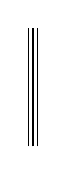
\begin{tikzpicture}\draw (0,0)--(0,1.5);\draw (.06,0)--(.06,1.5);\draw (.12,0)--(.12,1.5);\end{tikzpicture}}}
\mspage{14}

\scanpage{16}
\mspage{30}

\deleted{\deleted{pourra alors}\inserted{\unsure{faut donc}}
\deleted{\unsure{respecter}}\inserted{dans 3.9.} l'hypothèse \deleted{dans 3.9.}
avec : ``ou \deleted{\unsure{$B$ est lui-même un corps}}\inserted{$r(B)=r(A)B$}''
\deleted{(car grâce au résultat du et la}}

\uline{Corollaire} \inserted{4.}10. Soient $A$ un anneau local noethérien, de corps résiduel
$k$, $B_0$ une $k$-algèbre qui soit un anneau local noethérien, et soit une $k$-algèbre
de Cohen i.e. une $k$-algèbre formellement simple \deleted{pour sa} et complète
pour sa topologie ordinaire. Supposons de plus l'extension résiduelle $K/k$
séparable (ce qui n'est donc pas une restriction si $B_0=K$\deleted{\unsure{fini}}, mais en est
évidemment une en général). Alors il existe une $A$-algèbre topologique de
Cohen \inserted{$B$} qui se réduit suivant $B_0$, $B$ est unique à isomorphisme près
en vertu de \inserted{4.}8., et c'est un anneau noethérien local complet comme il se doit.

En vertu du théorème de structure \inserted{3.}4. on a $B_0\simeq K[[T_1,\ldots,T_n]]$,
et on est ramené, grâce au critère \inserted{4.}9. 2) et la transitivité de la
platitude, aux deux cas types: 1°) $B_0=K$ 2°) $B_0=k[[T_1,\ldots,T_n]]$. Dans
le premier cas, on utilise le résultat général de $0_{\mathrm{III}}$\inserted{10.3.1.}, et dans le
deuxième cas il suffit de prendre $B=\widehat{A}[[T_1,\ldots,T_n]]$.

\deleted{Théorème 3.1} \uline{Corollaire} \inserted{4.}11. Sous les conditions de 3.9.,
\inserted{si $k(B)/k(A)$ de multi. rad. finie,}
les conditions 1) et 2) équivalent aussi à: 3) $B$ est complet et formellement simple sur $A$

En effet, on sait déjà que \deleted{c'est nécessaire,}\inserted{$1)\longrightarrow3)$}
reste à prouver \deleted{la} $3)\Longrightarrow1)$
\deleted{suffisance} ou encore $3)\Longrightarrow2)$, i.e. on est ramené à prouver simplement que
$B$ est plat sur $A$. Or\unsure{n} faisant une extension de la base $A\longrightarrow A'$, $A'$ local
libre \inserted{de type fini} sur $A$ à extension radicielle convenable (cf $0_{\mathrm{III}}$), on trouve un $B'$
\inserted{local} sur $A'$ qui sera encore formellement simple sur $A'$, et de plus à extension
résiduelle \deleted{triviale} séparable. On dispose alors du théorème d'existence
\inserted{4.}10. qui nous garantit, grâce à \inserted{4.}8. (équiv de 0) et 1) ) que $B'$ est
Cohen sur $A'$ donc plat sur $A'$. Donc $B$ est plat sur $A$.

\margin{\figure{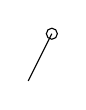
\begin{tikzpicture}\draw (0,0)--(.3,.6);\draw (.3,.6) circle (.07);\end{tikzpicture}}
(réduction \inserted{du NB} inutile dans le cas ``visé'')}

\mspage{15}

\scanpage{17}
\mspage{31}

En particulier, on obtient:

\uline{Corollaire} \inserted{4.}12. Soient $A\longrightarrow B$ un homomorphisme local d'anneaux locaux
noethériens, tel\deleted{s} que $\underline{r}(B)=\underline{r}(A)B$ et \deleted{que l'extens} soit $K/k$ l'extension
résiduelle. Conditions équivalentes: 1) $B$ est complet et formellement
simple sur $A$. 2) $B$ est \unsure{complet}, plat sur $A$, et $K/k$ est séparable.
3) $B$ est une algèbre de Cohen sur $A$. De plus, une extension séparable
$K$ de $k$ étant donnée, il existe une algèbre de Cohen $B$ sur $A$ se réduisant
suivant $K$, et $B$ est unique à isomorphisme de $A$-algèbres près.

La rédaction commence à faire un peu touffu, j'espère que tu pourras
la rendre plus lisible. D'ailleurs, je me répens un peu de la définition
\inserted{4.}7. telle quelle, il n'est pas vraiment naturel de supposer $B$ séparée
et complète pour sa topologie propre, mais simplement pour sa topologie
$IB$-adique (ce qui est moins fort); mais une telle modification demanderait
des réajustement analogues pour \inserted{4.}2., \inserted{4.}6. et la suite. Je t'en laisse
donc le choix, pensant que le choix adopté n'aura pas de grande importance
pratique pour la suite : dans \inserted{4.}9. à \inserted{4.}12. cela obligera simplement à
supprimer à certains endroits le mot ``complet'',
\inserted{ou \unsure{è|à} le remplacer par un autre \unsure{comple}}
\deleted{\deleted{en particulier ``Cohen'' deviendra} synonyme dans le contexte des anneaux locaux noethériens de
\deleted{``formellement} simple'', -- sous réserve de l'embêtante hypothèse de
\deleted{multiplicité} radicielle. \deleted{Il est vrai} Ce serait plutôt un avantage, \deleted{mais}
\deleted{il est vrai par contre que cela ne s'harmoniserait plus} de plus les
\deleted{anneaux de Cohen} sont}

\deleted{\uline{Corollaire \unsure{4.13}} $A\unsure{\longrightarrow|\text{---}} B$ hom loc. d'anneaux locaux
noeth, munis de leurs topologies naturelles. On
suppose $k(B)/k(A)$ à mult. \unsure{insép.} finie. Alors
Condit. \unsure{équivalentes}}

\mspage{16}

\scanpage{18}
\mspage{32}

\margin{\figure{\begin{tikzpicture}\draw (.2,0)--(0,0)--(0,5)--(.2,5);\end{tikzpicture}}}
\uline{Corollaire} \inserted{4.}13. Soit $A\longrightarrow B$ un homomorphisme local d'anneaux locaux
noethériens, on suppose $k(B)/k(A)$ à multiplicité radicielle finie
(par exemple une extension séparable, ou de type fini),
\inserted{ou $\underline{r}(B)=\underline{r}(A)B$.} \deleted{Conditions} On
munit $A$ et $B$ de leurs topologies habituelles. Alors les conditions suivantes
sont équivalentes: (i) $B$ est formellement simple sur $A$ (ii) $B$ est
plat sur $A$, et $B_0=B\otimes_A k\deleted{\unsure{A}}$ est une algèbre universellement régulière sur
$k$ (cf 2.6.).

En effet, les conditions (i) et (ii) étant invariantes par changement
de $B$ en $\widehat{B}$, on est ramené au cas où $B$ est complet, où cela est contenu
dans \inserted{4.}11. \inserted{resp. \unsure{3.12.|4.12.}} compte tenu que pour $B_0$, formellement simple = universellement
régulier en vertu de \inserted{3.}6.

Du point de vue pratique, les résultats du présent numéro consistent
essentiellement en \inserted{4.}13., \deleted{l'existence}\deleted{et} l'\uline{unicité} \deleted{de $B$} (moyennant les conditions
de \inserted{4.}13.) du $B$ correspondant à un $B_0$ donné, sous réserve que $B$ soit
complet pour la topologie $\underline{r}(A)$-adique (cette \deleted{unici} unicité étant un
corollaire immédiat d'ailleurs, puisqu'on dispose pour $B$ des deux propriétés
complémentaires formellement simple + plat),
\inserted{et enfin l'\uline{existence} moyennant la séparabilité de $K/k$.}
A force de dévissage et
de généralité, cette substance n'apparait pas assez clairement, et la
terminologie ``algèbre de Cohen'' introduite concurremment à ``formellement
simple'' risque \deleted{peut-être} d'embrouiller \inserted{plutôt} les idées (d'autant plus que nous
n'utiliserons plus jamais que ``formellement simple'' ). Aussi le présent
numéro rendra peut-être plus service si on commence à énoncer simplement
\inserted{4.}13. en théorème, avec le corollaire bien senti précédent, et qu'on
les démontre simultanément en deux pages ou trois, \deleted{avec} en laissant de
côté tout le fatras anneaux admissibles, algèbres de Cohen etc. Commencer
par l'existence d'un $B$ satisfaisant à la fois (i) et (ii) si $K/k$ est
séparable, se ramener à ce cas pour \inserted{4.}13. par descente comme dans \inserted{4.}11.
prouver \inserted{4.}13. alors par comparaison du $B$-type avec le $B$ donné, ce qui
donne en même temps l'unicité, et un point c'est tout.

\margin{(garder cependant 4.1. \uuline{au \unsure{N°1}})
On peut signaler 4.6. en remarque, pour réserver l'avenir.}
\margin{\figure{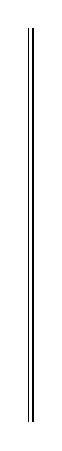
\begin{tikzpicture}\draw (0,0)--(0,5);\draw (.06,0)--(.06,5);\end{tikzpicture}}}

\mspage{17}

\scanpage{19}

Questions

\mspage{18}

\scanpage{20}

Questions ouvertes

1) Soit $A$ algèbre locale noethérienne sur $k$. Est-il vrai
que $A$ form$^t$ simple sur $k$ si $A$ est univ$^t$ régulière
sur $k$ [i.e., pour hom local $A\longrightarrow B$ d'anneaux
locaux noethériens, équivalence entre ``f$^t$ simple''
et ``univ. régulière'' \deleted{\unsure{sur}} sur $A$].

\margin{\unsure{OK}}

2) Soit $A$ algèbre locale noethérienne sur $k$, f$^t$
simple sur $k$ (pour sa topologie habituelle).
Est-il vrai que $A$ est f$^t$ simple pour sa topologie
discrète? \unsure{Cas où} $A$ est complet ? (Il est
possible que la réponse soit affirmative en
car $p>0$, négative en car 0). -- On peut
généraliser \unsure{au cas où on}. $A$ plat sur $\Lambda$,
\inserted{$A$ et} $\Lambda$ anneaux noethériens: si les
\unsure{localisés} de $A$ sont f$^t$ simples sur ceux de $\Lambda$
pour leur topologie habituelle, $A$ est-il f$^t$.
simple sur $\Lambda$ pour sa top. discrète.

\margin{Faux, \unsure{cf.} \unsure{valuation}
\unsure{$\checkmark$} \uline{\unsure{vrai;}} \uline{\unsure{possibilité}}
Peut-être \unsure{y a-t-il} \unsure{de l'espoir} \unsure{si on}
\unsure{on passe aux} extensions de $B$ \unsure{h.}
\deleted{\unsure{qui}} \unsure{qui sont}
en \unsure{anneaux} \uline{$\unsure{VA}$}
\unsure{(anneaux} à \unsure{résidu fini}).
\unsure{pas} \unsure{universelle} en \unsure{type fini}.}
\margin{\figure{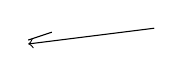
\begin{tikzpicture}\draw[->] (1.6,.2)--(0,0);\draw (0,.05)--(.3,.15);\end{tikzpicture}}}

3) $B$ \deleted{\unsure{libre}} \inserted{plat.} sur $A$, $A$ et $B$ noethériens.
Lieu des $\unsure{p}$ de $\operatorname{Spec}B$ dont l'anneau
local dans la fibre sur $\operatorname{Spec}A$ est f$^t$ simple
sur le corps résiduel en $A$, est-il ouvert?
\deleted{[NB. \unsure{Même}} (Si $B$ n'est pas plat sur $A$,

\mspage{19}

\scanpage{21}

\unsure{l'ens|lieu} des $p$ de $\operatorname{Spec}A$ où $B$ l'est est-il
ouvert? ]. Il \unsure{faudra|faut} supposer que $A$ et $B$
sont des ``bons anneaux''.

En particulier, l'\unsure{énoncé précédent} est-il
\deleted{$A,B$ \unsure{sont locaux}, $A\unsure{\longrightarrow|\text{---}}B$}
stable par localisation ?
\margin{Cf IV \unsure{2.10.1|2.40.1}}
\figure{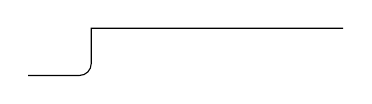
\begin{tikzpicture}\draw (0,0)--(.65,0) to[out=0,in=-90] (.8,.15)--(.8,.6)--(4,.6);\end{tikzpicture}}

\margin{On est ramené au cas où $A$ est \uline{intègre}; à \unsure{prouver}
(a) si $x\in U$, \unsure{pour} \unsure{tte} \unsure{générisation}
\unsure{au dessus de} $\unsure{x}$, $\unsure{x\longrightarrow y}$, $y\in U$.
(b) \deleted{Si $x\in U$, \unsure{son} \unsure{adhérence} \unsure{est} \unsure{contenue dans}}
\deleted{Si $x\in U$} $\unsure{U}$ est \unsure{dense en} $\unsure{\overline{\{y\}}}$,
\unsure{alors} \unsure{il} contient un \unsure{voisinage} de $\unsure{x}$
\unsure{dans} $\unsure{\overline{\{x\}}}$ \unsure{qui est dans} $U$.}
\margin{\figure{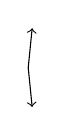
\begin{tikzpicture}\draw[<->] (0,1)--(-.05,.5)--(0,0);\end{tikzpicture}}}

Le cas d'extensions résiduelles finies.
cf critère jacobien de Nagata et
th. de Nagata pour une algèbre locale noeth
complète sur un \uline{corps}.

OK. en caractéristique 0 pour les \uline{bons
anneaux}, grâce à la \uline{résolution des
singularités}.

\margin{Pour (b), dans le cas d'un bon anneau,
on est ramené au cas où $B$ est \uline{régulier}. \unsure{Alors},
\unsure{a)} \unsure{reste une} \unsure{hypothèse de}
la résolution des singularités, et
\unsure{pour a)} \unsure{se résout par} \uline{l'affirmative}.
\unsure{En réalité}, il se résout par l'affirmative
pour les bons anneaux, \uline{en \unsure{caractéristique} \unsure{entière|quelconque}},
\uline{\unsure{pourvu qu'on sache}}
\unsure{que le} \unsure{lieu où} un $f$ sur $X$
est \unsure{géométriquement} \unsure{régulier}
est \uline{ouvert} (au \unsure{moins} \unsure{au-dessus de} $k$).}

4) $A\unsure{\text{---}|\longrightarrow}B$ hom d'anneaux
noeth. Lieu des $\unsure{q|p}$ de
$\operatorname{Spec}B$ en lesquels $B$ est plat
sur $A$ est-il ouvert?
[Ceci revient à vérifier
que pour $\forall p\in\operatorname{Spec}A$,
et $\forall q$ au dessus de $p$,
maximal parmi \unsure{ceux-là|ceux-ci},
posant $A'=A/p$, $B'=B/q$
\inserted{$A'\subset B'$ intègres}
[\unsure{donc} $B'\otimes_{A'}K'$ \unsure{est un corps}]
$\exists$ un ouvert non vide de $\operatorname{Spec}B'$
en \unsure{lesquels|lequel} $B'$ est plat sur $A'$.
\figure{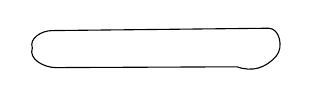
\begin{tikzpicture}\draw (0,.2) to[out=110,in=180] (.25,.42)--(3,.45) to[out=0,in=50] (3.1,.1) to[out=230,in=-20] (2.6,-.04)--(.3,-.05) to[out=180,in=-110] (0,.2);\end{tikzpicture}}

\begin{center}
M. DUFOUR\\
VARITYPISTE\\
131, RUE LECOURBE\\
PARIS XV$^{\mathrm e}$\\
\figure{\begin{tikzpicture}\fill (0,0) rectangle (.12,.12);\end{tikzpicture}}\\
C. C. P. Paris \unsure{14.143.34|14.143-34}\\
R. M. 140.029
\end{center}

\mspage{20}

\scanpage{22}

\deleted{M. DUFOUR\\
VARITYPISTE\\
131, RUE LECOURBE\\
PARIS XV$^{\mathrm e}$\\
\figure{\begin{tikzpicture}\fill (0,0) rectangle (.12,.12);\end{tikzpicture}}\\
C. C. P. Paris 14.143-34\\
R. M. 140.029}
\figure{\begin{tikzpicture}\draw (0,1.6)--(.7,0);\draw (1.1,1.5)--(1.7,.65);\draw (1.8,1.5)--(1.95,1.05);\end{tikzpicture}}

$A$ algèbre \inserted{locale noeth. complète,}
f$^t$ simple sur $k$ pour sa
topologie habituelle, alors $A$
est-il f$^t$ simple sur $\unsure{K|k}$ pour sa
topologie discrète ???.
\figure{\begin{tikzpicture}\draw (0,0)--(0,.5) to[out=90,in=180] (.2,.7)--(2.6,.7) to[out=0,in=10] (2.55,.8);\end{tikzpicture}}

\deleted{1°) Cas $p>0$}
On se \unsure{ramènera|ramène} au cas où $k$ est le
corps premier (plus gén. un corps \uline{parfait})
\inserted{\unsure{ou même} où $K/k$ est séparable, $K$ \unsure{le c. résiduel}}

\deleted{\unsure{1°)} \uline{Cas $\unsure{p>0|p=0}$}}
\unsure{Alors on a.}
$A\simeq K[[t_1,\ldots,t_n]]$, $K/k$
une extension \uline{séparable}.
\deleted{$\unsure{K}$ est form$^t$ simple sur
$k$, il suffira que $A$ le soit sur $K$.}
\deleted{$\unsure{K}$}

\unsure{1°)} \uline{Cas $p>0$}

Supposons que $K/k$ a une $p$-base
\uline{finie}, i.e.
\margin{$\Omega_{K/k}$ est fini sur $K$.}

\deleted{Si $K$ est parfait, alors}
\deleted{Alors $A$ est un anneau}

\deleted{$A$, ayant une $p$-base \inserted{$(t_1,\ldots,t_n)$},
sur $K$, est f$^t$ simple sur $K$.}
\deleted{\unsure{ayant une $p$-base},}
\deleted{\unsure{Il suffit} de connaître une
$p$-base de $A$ sur $k$. Il en existe si
$K$ est fini sur $K^p$, on prend une $p$-base
$(x_1\unsure{\text{--}|,}\,x_{\unsure{m|n}})$ de $K$, et y adjoint $t_1,\ldots,t_n$.}
\figure{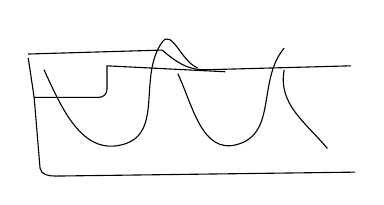
\begin{tikzpicture}[x=.5cm,y=.5cm]
\draw (0,3.1)--(3.4,3.2) to[out=-40,in=180] (4.5,2.7)--(8.2,2.8);
\draw (0,3)--(.15,2)--(1.8,2) to[out=0,in=-90] (2,2.2)--(2,2.8)--(5,2.65);
\draw (.4,2.7) to[out=-65,in=195] (2.4,.8) to[out=15,in=-125] (3.4,3.4) to[out=55,in=160] (4.3,2.75);
\draw (3.8,2.6) to[out=-65,in=195] (5.3,.8) to[out=15,in=-130] (6.5,3.25);
\draw (6.5,2.7) to[out=-100,in=130] (7.6,.7);
\draw (.15,2)--(.3,.2) to[out=-80,in=180] (.7,0)--(8.3,.1);
\end{tikzpicture}}

En la complétant par les $t_i$, on trouve
une $p$-base de $A$ sur $k$, et $K(A^p)=K\otimes_{K^p}A^p$.
[cf ``\unsure{Diff.}'']. Donc dans ce cas \unsure{on gagne}.

\mspage{21}

\scanpage{23}

\deleted{\unsure{2°}}) \uline{Cas contraire}. Je suis pessimiste.

2°) Cas $p=0$. Par contre $k[[t]]$ sur $k$,
($k=\mathbb Q$, ou $k=\mathbb C\ldots$). Je présume que
si $\dim A\unsure{\geq|>}0$, $A$ n'est jamais \unsure{for}$^t$ simple
sur $k$ pour sa topologie discrète.

Dans les cas défavorables, je doute qu'il
y ait \unsure{un} ``\unsure{form}$^t$ simple contenant un corps
premier'' [si $k$ n'est pas alg. sur le sien].

$\Omega_k\otimes_k A\longrightarrow\Omega_A$
admet un inverse à gauche ?

\deleted{Supposons $k$ \unsure{le degré de} $\unsure{\Omega_k|\Omega^-_k}$}
\[
k=\mathbb Q\bigl((x_i)_{i\in I}\bigr)
\qquad \deleted{\unsure{k=\mathbb Q}}
\]
\[
A=k[[\unsure{t|u}]],\qquad
\Omega_k\otimes_k A\simeq A^{(I)}
\unsure{=}\deleted{\prod}\inserted{\unsure{\bigoplus_{i\in I}}}
A\,d_{/\mathbb Q}x_i,
\]
on cherche $A\unsure{\mathrel{\overset{D}{\text{---}}}|\xrightarrow{D}}\Omega_k\otimes_k A$, qui soit
donné sur $k$ par $D(x_i)=d_{/\mathbb Q}x_i$.
Or s'il y a un tel $D$, alors $Dt$ est combinaison lin.
finie de certains $d_{/\mathbb Q}x_i$, $i\in J$, et \unsure{remplaçant}
$\mathbb Q$ par $k_0=\mathbb Q\bigl((x_i)_{\unsure{i\in J}}\bigr)$,
on peut supposer que
$dt=0$.
\deleted{$D(\sum a_i t^i)=$}

\mspage{22}

\scanpage{24}

\uline{Proposition}. Soient $k$ un corps, $K$ une extension
telle que $\Omega_{K/k}$ soit de dim infinie sur
$K$, et $A\inserted{=K[[t_1,\ldots,t_n]]}$ une algèbre de séries formelles
sur $K$, avec $n>0$. Alors $A$, muni de sa
topologie \uline{discrète}, n'est pas f$^t$ simple sur $K$
\unsure{relativement} à $k$, et à fortiori n'est pas f$^t$ simple sur $k$.
\margin{\figure{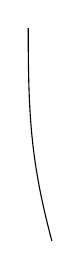
\begin{tikzpicture}\draw (0,2.7) to[out=-90,in=105] (.3,0);\end{tikzpicture}}}

Il faut prouver que l'hom
\[
\Omega_{K/k}\otimes_K A\unsure{\text{---}|\longrightarrow}\Omega_{A/k}
\]
n'a pas d'inverse à gauche, i.e. qu'il
n'existe pas de dérivation
\[
D:A\unsure{\text{---}|\longrightarrow}\Omega_{K/k}\otimes_K A
\]
qui sur $K$ induise $d_{K/k}\otimes_K\unsure{1_A}$. Or
si on avait une telle $D$, alors les
$D(t_i)$ \unsure{seront|seraient} dans un sous-module
$V\otimes_K A$, $V\subset\Omega_{K/k}$ de dim finie, donc
il existerait une \unsure{coextension|extension} de \uline{type fini}
$k'$ de $k$, telle que les $Dt_i$ soient dans
$\operatorname{Im}\Omega_{k'/k}\otimes_{k'}A$, donc leurs images dans
$\Omega_{K/k'}\otimes_K A$ \unsure{seront|seraient} nulles. \unsure{Donc quitte}
à remplacer $k$ par $k'$, [ce qui
ne change pas \unsure{l'hyp. !}] on peut supposer

\deleted{M. DUFOUR\\
VARITYPISTE\\
131, RUE LECOURBE\\
PARIS XV$^{\mathrm e}$\\
\figure{\begin{tikzpicture}\fill (0,0) rectangle (.12,.12);\end{tikzpicture}}\\
C. C. P. Paris 14.143-34\\
R. M. 140.029}
\figure{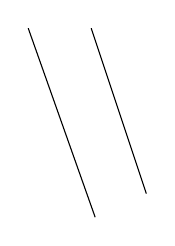
\begin{tikzpicture}\draw (0,2.4)--(.85,0);\draw (.8,2.4)--(1.5,.3);\end{tikzpicture}}

\mspage{23}

\scanpage{25}

les $Dt_i=0$. \deleted{\unsure{Alors}} Prenons une
\uline{base} de $\Omega_{K/k}$ sur $K$, \unsure{soit} $(\omega_i)_{i\in I}$,
donc $\Omega_{K/k}\otimes_K A\simeq A^{(I)}\subset A^I$. En tant
que dérivation dans $A^I$, $D$ est donnée
par ses composantes $D_i$, qui sont
\unsure{uniq}$^t$ déterminées
\[
D_i\Bigl(\sum_\lambda a_\lambda t^\lambda\Bigr)
=\sum_\lambda \unsure{d^i_{K/k}|d_{K/k}^{\,i}}(a_\lambda)t^\lambda
\]
Il reste à prouver qu'on peut trouver
des $f=\sum a_\lambda t^\lambda$ telles que les
\[
\bigl(D_i(\unsure{f|\varphi})\bigr)_{i\in I}\notin A^{(I)}.
\]
\deleted{Il suffit}
\inserted{Choisissons}
\deleted{pour ceci \unsure{que} \inserted{\unsure{pour avoir}} \unsure{les}
$D_i(a_\lambda)$ \unsure{pour} $\unsure{\forall}$}
\deleted{de \unsure{trouver}}
une \uline{suite infinie} $i_0,i_1,\ldots,i_n$
d'indices distincts de $I$, \deleted{telle que} pour $\unsure{\forall}$
\deleted{$D_{i_n}(a_n)\ne0$}
\unsure{n} il existe $a_n\in K$ tel que
\deleted{$\unsure{D_{i_n}(a_n)\ne0}$},
\deleted{\unsure{(ceci est possible}}
$d_{K/k}a_n^{\unsure{i_n}}\ne0$, il suffit alors de
prendre $f=\sum a_nt^n$. .\,.\,.\,.\,.

\mspage{24}

\scanpage{26}

\deleted{Différentielles}

\mspage{25}

\scanpage{27}

\uline{Remarque}. Soient
\diagram{\begin{tikzcd}[ampersand replacement=\&]
k \arrow[r] \arrow[d,dash] \& K \arrow[d,dash] \\
k'=k\cap K^p \arrow[r,dash] \& K^p
\end{tikzcd}}
alors deux éléments $\unsure{x},y$ de $k$ peuvent être
$p$-indépendants \inserted{dans $\unsure{k|K}$ sur}
\deleted{\unsure{sur $k$}} $k\cap K^p$, et non
\inserted{dans $K$} sur $K^p$,
i.e. $d_{k/k'}x$ et $d_{k/k'}y$ peuvent être lin. indépendants,
sans que $d_{K/K^p}x$ et $d_{K/K^p}y$ le soient.
\uline{à fortiori}, $\Omega^1_{k/k\cap K^p}\otimes_k K\to\Omega^1_K$
peut n'être pas injectif, ou \deleted{\unsure{encore}} ce qui revient
au même, il peut arriver que le noyau \inserted{$N_{K/k}$}
de $\Omega_k\otimes_k K\unsure{\text{---}|\to}\Omega_K$ ne soit pas engendré sur $K$
par les $dx\otimes1$ $(x\in k\cap K^p)$.
\inserted{\uline{\unsure{qui est} \unsure{évident.} \unsure{(donc}}}

\margin{$\Omega^1_{k\cap K^p/\unsure{k^p}}\otimes_{k\cap K^p}K
\to\Omega^1_k\otimes_k\unsure{K}\to\Omega^1_K$}
\margin{N.B. \deleted{\unsure{Alors}} (\unsure{l'existence|l'assertion}
\unsure{ci-dessus}) \deleted{\unsure{à déterminer}}
\unsure{revient} \deleted{\unsure{pour}} que $N_{K/k}$
\deleted{\unsure{peut}} \unsure{n'être} ``défini sur $k$'' !
On peut \unsure{prendre} un premier \unsure{exemple} où il est
de dim \uline{1} \unsure{déjà}.}
\figure{\begin{tikzpicture}[x=1cm,y=1cm]
\draw (0,0) .. controls (.4,.5) and (.8,-.15) .. (1.2,0)
.. controls (3,.2) and (7,-.25) .. (9.3,.05)
.. controls (10,.2) and (10.8,.1) .. (11,.65);
\draw (10.85,.62)--(11,.65)--(10.94,.49);
\draw (8.2,.4) .. controls (7.65,.8) and (7.9,1.15) .. (8.5,1.18)
--(10.25,1.31);
\end{tikzpicture}}

Voici un contre. Soit $\mathbb F$ le corps premier
[ou un corps parfait quelc.], \uuline{$x,y,a_i$}
\inserted{$(1\le i\le p-1)$} des indéterminées sur $\mathbb F$,
\unsure{on pose} \deleted{$\unsure{\beta=y-\alpha x}$}
\[
\deleted{K^p=\mathbb F(x^p,\unsure{y^p},\unsure{\alpha})
\qquad\text{donc}\quad K=\mathbb F(x,\unsure{y},\unsure{\alpha^{1/p}})}
\]
\deleted{$\unsure{k'}=$}
\[
\left\{\begin{aligned}
a_0&=y-\sum_1^{p-1}a_i x^i\\
a&=x^p
\end{aligned}\right.
\qquad \text{soit}\quad y=\sum_0^{p-1}a_i x^i
\]
\[
K^p=\mathbb F(a,a_0,\unsure{a_1,\ldots,a_{p-1}})
=\deleted{\mathbb F(\unsure{\alpha},x^p,y-\alpha x)}
\inserted{\mathbb F\Bigl(x^p,a_1,\ldots,a_{p-1},y-\sum_1^{p-1}a_i x^i\Bigr)}
\]
\[
\deleted{K=\mathbb F(\alpha^{1/p},x,(y-\alpha x)^{1/p})}
\qquad\text{i.e.}\quad K=\mathbb F(x,a_1^{1/p},\ldots,a_{p-1}^{1/p},(\text{''})^{1/p})
\]
\[
k=\mathbb F(x,y)
\]
\margin{NB $a$ et $(a_i)_{0\le i\le p-1}$ sont alg. ind. sur $\mathbb F$.}
\figure{\begin{tikzpicture}[x=1cm,y=1cm]
\draw (2.8,1.2) .. controls (3.1,1.2) and (2.9,.85) .. (3.12,.8)
.. controls (3.3,.75) and (3.1,.5) .. (3.2,.3)--(2.9,.25);
\draw (.9,.08)--(2.65,.35);
\end{tikzpicture}}
\margin{[N.B. $x,\unsure{z}\in K$, donc $y=\unsure{\alpha x+\beta}\in K$,
donc $\unsure{k}\subset K$}

\mspage{26}

\scanpage{28}

\unsure{sur} des répartitions sur $K$. Pour un \uline{idèle} $I'$ de $K'$,
$\operatorname{Ext}_{K',K}(I')$ est un \unsure{idèle}
de $K$. En ce qui concerne les répartitions \uline{principales}, l'extension à $K$ de \unsure{celle}
attachée à $x'\in K'$ est la répartition principale de $K$ attachée à $x'$ \unsure{considéré}
comme élément de $K$. Pour un idèle $I'$ de $K'$ on a
\mspage{27}
\[
(39)\quad \operatorname{Ext}_{K',K}(D'(I'))=D(\operatorname{Ext}_{K',K}(I'))
\quad\text{(``extension du diviseur''=``diviseur de l'extension'').}
\]

Enfin une formule évidente de transitivité.

Etant donnée une répartition $X=(x_{\unsure{P|p}})$ sur $K$, on appelle \uline{trace} et \uline{norme} de $K$ à
$K'$ de $X$, et on note $\operatorname{Tr}_{K/K'}(X)$ et $N_{K/K'}(X)$ les répartitions $(a_{\unsure{P'|p'}})$ et $(b_{\unsure{P'|p'}})$ de
$K'$ définies par
\[
(40)\quad a_{\unsure{P'|p'}}=\sum_{\unsure{P|p}\unsure{\mid|/}\unsure{P'|p'}}\operatorname{Tr}_{\widehat K_{\unsure{P|p}}/\widehat K'_{\unsure{P'|p'}}}(x_{\unsure{P|p}})
\qquad\text{et}\qquad
b_{\unsure{P'|p'}}=\prod_{\unsure{P|p}\unsure{\mid|/}\unsure{P'|p'}}N_{\widehat K_{\unsure{P|p}}/\widehat K'_{\unsure{P'|p'}}}(x_{\unsure{P|p}}).
\]
D'après les formules (12) et (13) (§ 2,n°2) les restrictions de $\operatorname{Tr}_{K/K'}$ et
$N_{K/K'}$ aux répartitions \uline{principales} (identifiées aux éléments de $K$) coïncidant
avec les applications $\operatorname{Tr}_{K/K'}$ et $N_{K/K'}$ définies pour les éléments de $K$. Il est
clair que l'application $\operatorname{Tr}_{K/K'}$ est une \uline{application} $K'$-\uline{linéaire} de l'ensemble
des répartitions de $K$ dans celui de $K'$, pour leurs structures d'espaces vectoriels sur $K'$.
La norme d'un \uline{idèle} de $K$ est un idèle de $K'$, et l'application
$N_{K/K'}$ est un \uline{homomorphisme} du groupe multiplicatif $J_K$ dans le groupe multiplicatif $J_{K'}$.
On a enfin les formules suivantes (que l'on vérifie comme l'âne
qui trotte) :
\[
\begin{aligned}
(41)\quad&\operatorname{Tr}_{K/K'}(z.\operatorname{Ext}_{K',K}(X'))=(\operatorname{Tr}_{K/K'}(z)).X'
\quad\text{pour }z\in K.\\
(42)\quad&\operatorname{Tr}_{K/K'}(\operatorname{Ext}_{K',K}(X'))=n.X'.\\
(43)\quad&N_{K/K'}(\operatorname{Ext}_{K',K}(X'))=(X')^n.\\
(44)\quad&D'(N_{K/K'}(I))=N_{K/K'}(D(I))\quad\text{pour tout idèle }I\text{ de }K.\\
(45)\quad&\text{formules de transitivité.}
\end{aligned}
\]

\uline{5 . Topologies sur l'espace des répartitions et sur le groupe des idèles} .

Soit $(G_\alpha)$ une famille de groupes topologiques, $(H_\alpha)$ une famille se dous-groupes
\uline{ouverts distingués} de $G_\alpha$. Sur le groupe produit $G=\prod_\alpha G_\alpha$ on met la topologie
pour laquelle un système fondamental de voisinages de l'élément neutre est for-

\mspage{27}

\scanpage{29}

\deleted{\unsure{Il faut bien} $x,y\notin$}
\margin{\unsure{cf le NB en final}}
\figure{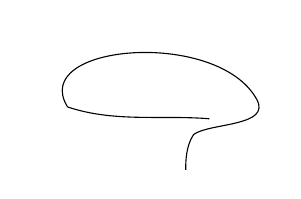
\begin{tikzpicture}\draw (0,0) .. controls (-.5,.8) and (1.9,1) .. (2.4,.1)
.. controls (2.6,-.25) and (1.8,-.2) .. (1.6,-.35)
.. controls (1.5,-.5) and (1.5,-.7) .. (1.5,-.8);
\draw (0,0)..controls(.6,-.2)and(1.2,-.1)..(1.8,-.15);\end{tikzpicture}}
Par construction, on a $x\in K$, $x\notin K^p$, et
$y\notin K^p$, $y\in K^p(x)$, avec \deleted{$\unsure{\alpha,\beta}$}
\inserted{les $a_i$} sont les \uline{seuls} $\in K^p$
tels qu'on ait \deleted{$y=\alpha x+\beta$. \unsure{Evident}}
\inserted{$y=\sum_0^{p-1}a_i x^i$}.

Comme $x\notin K^p$, on a $x\notin K^p\cap k$, mais bien
sur $x^p\in K^p\cap k$ ; si donc $(x,y)$ \unsure{n'étaient}
\deleted{lin.} $p$-\unsure{libres} sur $K^p\cap k$, on aurait une
relation $y=\sum_0^{p-1}a_i' x^i$, les $a_i'\in K^p\cap k$, donc
\deleted{\unsure{les}} \inserted{on aurait} $a_i'=a_i$, donc
$a_i\in k=\mathbb F(x,y)$, absurde.

N.B. Condition essentielle
\[
\left\{\begin{array}{l}
(x,y)\quad p\text{-libres sur }\lambda=\mathbb F(a_1,\ldots,a_{p-1})\\
\deleted{\unsure{a_1}}\quad\lambda\unsure{\notin|\not\subset}\mathbb F(x,y)
\end{array}\right.
\]
\deleted{Il suffit \unsure{par}}
exemple
\deleted{que $x,y$ \unsure{soient} \inserted{\unsure{$p$-indépendants}}
\unsure{sur} $\lambda=\mathbb F(a_0,\ldots,a_{p-1})$, et
\unsure{que prendre} $\lambda$ \unsure{en un autre}]
\inserted{\unsure{de} $\mathbb F(x,y,a)$}}

Prendre $x,y,a_1$ \deleted{\unsure{alg.}} $p$-indép. sur $\unsure{\mathbb F_p|\mathbb F_0}$ et prendre
$a_i=0$ pour $1<i\le p-1$. Bien entendu, $F$ peut
être n'importe quel corps parfait \unsure{dans la sc.}
On peut aussi prendre $x,y$ alg. indép. sur $F$,
et $a_1$ alg. \deleted{\unsure{séparable}} \inserted{\unsure{irrationnel}} sur $F$, $a_1\notin F$, alors
$K$ est obtenu \unsure{en adjoignant} une racine
$p$-ième (celle de $y-ax$) dans $k(b)$, où $b$ est
alg. \unsure{séparable} sur $k$ $[b=a^{1/p}]$.

\mspage{28}

\scanpage{30}

Etant donné un diviseur $D'=\sum_{P'}m(P').P'$ de $K'$, nous appellerons \uline{extension} \unsure{de}
$D'$ à $K$ et noterons $\operatorname{Ext}_{K',K}(D')$ le diviseur de $K$ défini par
\mspage{29}
\[
(31)\quad\operatorname{Ext}_{K',K}\Bigl(\sum_{P'}m(P').P'\Bigr)
=\sum_{P'}m(P').\Bigl(\sum_{P\mid P'}e(P).P\Bigr).
\]
Il est clair que $\operatorname{Ext}_{K',K}$ est un \uline{isomorphisme croissant} du groupe
\deleted{\unsure{des}} ordonné des diviseurs de $K'$ dans celui des diviseurs de $K$.
En vertu de (29) on a
\[
(32)\quad\operatorname{Ext}_{K',K}(D'(x'))=D(x')\quad\text{pour }x'\in K'.
\]
Si $K''\subset K'\subset K$, et pour tout diviseur $D''$ de $K''$,on a
\[
(33)\quad\operatorname{Ext}_{K',K}(\operatorname{Ext}_{K'',K'}(D''))
=\operatorname{Ext}_{K'',K}(D'').
\]
Etant donné un diviseur $D=\sum_P m(P).P$ de $K$, nous appellerons \uline{norme} de $K$ à $K'$ \unsure{de}
$D$, et noterons $N_{K/K'}(D)$ le diviseur de $K'$ défini par
\[
(34)\quad N_{K/K'}(D)=\sum_{P'}\Bigl(\sum_{P\mid P'}m(P)\uline{f(P)}\Bigr).P'.
\]
Il est clair que $N_{K/K'}$ est un \uline{homomorphisme croissant} du groupe ordonné des diviseurs
de $K$ dans celui des diviseurs de $K'$. Comme $\sum_{P\mid P'}e(P)f(P)=n$, on voit que
\[
(35)\quad N_{K/K'}(\operatorname{Ext}_{K',K}(D'))=n.D'.
\]
D'autre part (30) montre que l'on a
\[
(36)\quad D'(N_{K/K'}(x))=N_{K/K'}(D(x))\quad\text{pour tout }x\in K.
\]
Enfin, si $K''\subset K'\subset K$, et si $D$ est un diviseur de $K$, on a
\[
(37)\quad N_{K'/K''}(N_{K/K'}(D))=N_{K/K''}(D).
\]
Supposons maintenant que $\unsure{\overline\Phi'}$ satisfasse à une formule du produit
$\prod_{P'}(f_{P'}(x'))^{r(P')}=1$.
Alors, en vertu de (30), $\unsure{\overline\Phi}$ satisfait à la formule
du produit $\prod_P(f_P(x))^{r(P)}=1$, où $r(P)=f(P)r(P')$ pour $P\mid P'$.
D'après la définition des \uline{degrés} des diviseurs, et comme
$\sum_{P\mid\unsure{P|P'}}e(P)f(P)=n$, on a, pour tout couple de diviseurs $D'$ de $K'$ et $D$ de $K$ :
\[
(38)\quad d(\operatorname{Ext}_{K',K}(D'))=n.d(D')\qquad\text{et}\qquad d(N_{K/K'}(D))=d(D).
\]
Etant donnée une \uline{répartition} \deleted{$\unsure{X'=(x'_P)}$}
$X'=(x'_{P'})$ $(x'_{P'}\in\widehat K'_{P'})$, nous appellerons
\uline{extension} de $X'$ à $K$ et noterons $\operatorname{Ext}_{K',K}(X')$ la répartition sur $K$ définie par
$X=(x_P)$, où, pour $P\mid P'$, l'élément $x_P$ de $\widehat K_P$ est $x'_{P'}$.
Il est clair que l'application $\operatorname{Ext}_{K',K}$ est un \uline{isomorphisme} de l'anneau des répartitions sur $K'$ dans ce

\mspage{26}

\cotefile{23}
\scanpage{2}

EGA $\overline{\underline{\mathrm{IV}}}$, Calcul diff.

(Compléments)

\mspage{1}

\scanpage{3}

Discriminant etc

\mspage{2}

\scanpage{4}

$E$ faisceau loc. libre de rang $r+1$ sur $S$

$P=P(E)$ fibré projectif associé, on a une suite exacte canonique
\diagram{\begin{tikzcd}[ampersand replacement=\&]
0\arrow[r]\&\Omega^1_{P/S}\arrow[r]\&g^*(\underline E)(-1)\arrow[r,dash]\&\underline O_P\arrow[r,dash]\&0
\end{tikzcd}}

[qui donne un isom can
\[
(1)\qquad\Omega^r_{P/S}\xrightarrow{\sim}g^*\Bigl(\bigwedge_{\underline O_S}^{r+1}E\Bigr)(-r-1)
\qquad]
\]

Si donc $X$ est un sous-schéma de $P$ \unsure{lisse} sur $S$, de dim relative \inserted{$(n=$}$r-p$
associé au faisceau \deleted{loc. libre} \inserted{d'idéaux} $J$, on a la suite exacte
\diagram{\begin{tikzcd}[ampersand replacement=\&]
0\arrow[r,dash]\&J/J^2\arrow[r]\&\Omega^1_{P/S}\otimes\underline O_X\arrow[r]\&\Omega^1_{X/S}\arrow[r]\&0
\end{tikzcd}}
d'où l'isomorphisme
\[
(2)\qquad\Omega^r_{P/S}\otimes\underline O_X
\xleftarrow{\sim}\Omega^{\unsure{n}}_{X/S}\otimes\bigwedge_{\underline O_X}^p(J/J^2)
\]
d'où en composant (1) et (2), désignant par $f:X\unsure{\text{---}|\to}S$
le morphisme structural
\[
\deleted{\unsure{\Omega^r}}
f^*\Bigl(\bigwedge_{\underline O_S}^{r+1}\underline E\Bigr)(-r-1)
\xleftarrow{\sim}\Omega^{\unsure{n}}_{X/S}\otimes\bigwedge_{\underline O_X}^p(J/J^2)
\]

Supposons que $X$ soit une intersection complète, définie
par un sous-module \inserted{gradué $M$} loc. facteur direct de
$\operatorname{Symm}^*(\underline E)$,
\deleted{[qui est \unsure{un}} loc. libre de rang $p$
[$\unsure{\text{il n'est}}$ \deleted{défini}
déterminé que modulo le carré $\underline I^2$ de l'Idéal qu'il
définit ; mais sa structure est canonique]. On a
un hom., si $I_d$ est la composante de degré $d$ de $I$
\[
g^*(I_d)(-d)\longrightarrow J
\]
d'où des hom \uline{surjectifs}
\[
\coprod g^*(M_d)(-d)\unsure{\text{---}|\longrightarrow}J
\]
induisant un \uline{isom}
\[
\coprod f^*(M_d)(-d)\xrightarrow{\sim}J/J^2\simeq\operatorname{Conormal}_{P/X}
\]

\mspage{3}

\scanpage{5}

Par suite, on a
\[
\bigwedge_{\underline O_X}^p J/J^2\simeq
f^*\Bigl(\bigotimes_i\bigwedge^{\alpha_i}M_{d_i}\Bigr)(-\sum\alpha_i d_i)
\]
où $M_{d_i}$ sont les composantes non nulles de $M$, supposées
de \unsure{degré} $\alpha_i$. D'où un isom
\[
\Omega^n_{X/S}\otimes f^*\Bigl(\bigotimes_i\bigwedge^{\alpha}M_{d_i}\Bigr)(-\sum\alpha_i d_i)
\xrightarrow{\sim}f^*\Bigl(\bigwedge_{\unsure{S|\underline O_S}}^{r+1}\underline E\Bigr)(-r-1)
\]
[Comprendre : un hom qui existe en tous cas dès
qu'on se donne des $M_{d_i}\to\operatorname{Symm}^{d_i}(\underline E)$, les $M_{d_i}$ loc.
libres de rang $\alpha_i$, et $X$ défini par
\inserted{l'idéal engendré par} les images
des $M_{d_i}$, posant $p=\sum\alpha_i$, $n=r-p$], i.e. on a
\[
\Omega^n_{X/S}\xrightarrow{\sim}
f^*\Bigl(\bigl(\bigwedge_S^{r+1}E\bigr)\otimes
\bigl(\bigotimes_i\bigwedge^{\alpha_i}\check M_{d_i}\bigr)\Bigr)
(\sum\alpha_i d_i-r-1)
\]

Dans le cas où
\[
\sum\alpha_i d_i=r+1
\]
on trouve donc
\[
\Omega^n_{X/S}\xrightarrow{\sim}f^*(-)
\]

Supposons p.ex. que $E$ soit le faisceau loc. libre de
rang $3$ associé à une courbe elliptique lisse
sur $S$, donc $r=2$, il n'y a qu'un seul $M_{d_i}$, $d_i=3$,
$\alpha_i=1$, on trouve
\[
\Omega^1_{X/S}\xrightarrow{\sim}f^*\bigl(\bigwedge^3E\otimes\check M\bigr)
\]
Or $E$ a une filtration de facteurs $\underline O_S$,
\deleted{$\unsure{g}$} $\mathcal L^{\otimes2}$, $\mathcal L^{\otimes3}$,
où $\mathcal L$ est inversible \unsure{tel que}
$f^*(\mathcal L)\simeq\unsure{\mathcal T}_{X/S}$, donc
$\bigwedge^3E\simeq\mathcal L^{\otimes5}$, et comme
$\Omega^1_{X/S}\simeq f^*(\check{\mathcal L})$, on aura
\[
\check{\mathcal L}\xrightarrow{\sim}\mathcal L^{\otimes5}\otimes\check M
\qquad\text{d'où}\qquad M\xrightarrow{\sim}\mathcal L^{\otimes6}.
\]

\mspage{4}

\scanpage{6}

\diagram{\[\begin{array}{cc}
E&\operatorname{Symm}_k(\overset{\deleted{\unsure{\vee}}}{E})^{\vee}\\
P^r&\Phi^k(P^r).
\end{array}\]}
\[
\unsure{\delta}_{r,k}\in\Phi^{(k-1)(r+1)}\bigl(\Phi^k(P^r)\bigr)
\]
(discriminant)

défini au signe près

\margin{$\underbrace{k-1\quad k-1\qquad k-1}_{r+1\ \text{fois}}$
\quad $(k-1)(r+1)$}

section de $\underline O_{\Phi^k(P^r)}((k-1)(r+1))$

Considérons une section \inserted{$\varphi$} de $\Phi^k(P^r)$ sur $S$, elle
définit donc un \deleted{\unsure{hom.} $\Phi^k(P^r)$ \unsure{section de}}
faisceau inversible $\check M$ sur $S$, image inverse
de $\underline O_{\Phi^k(P^r)}(1)$] et
\deleted{\unsure{si} l'image \unsure{la section}}
\inserted{$\delta_{r,k}$ a comme}
\deleted{$M$ \unsure{est engendré par la}}
l'image réciproque une section \inserted{$\delta$} de
$\check M^{(k-1)(r+1)}$.
\margin{quotient de $\operatorname{Symm}_k(E)^\vee$,
\unsure{i.e. dual d'un} sous-faisceau $M$ \unsure{qui est facteur}
\unsure{de} $\operatorname{Symm}_k(E)$}
\figure{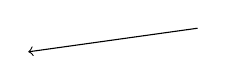
\begin{tikzpicture}\draw[->](2.4,.2)--(.25,-.1);\end{tikzpicture}}
Donc la section $\varphi$ \unsure{se remonte}
par $\Phi^k(P^r)_{\delta_{r,k}}$, i.e. $P^r_\varphi$ est \unsure{lisse} sur $S$,
sss $\delta$ est partout non nulle. Notons que
d'ailleurs, si $J=J_\varphi$ est l'idéal défini par $\varphi$
sur $P^r$, on a
\[
J\deleted{\unsure{_\varphi}}\simeq g^*(\overset{\deleted{\unsure{\vee}}}{M})(-k)
\]
\margin{\unsure{dualisons ici} $M\quad\check M$}
\figure{\begin{tikzpicture}\draw(0,0)..controls(.8,-1)and(.2,1.8)..(.65,1.2)
..controls(1,-.2)and(1.3,.2)..(1.45,1)
..controls(1.7,.3)and(2,.8)..(2.15,.9)
..controls(2.45,1.2)and(2.7,.7)..(2.9,.95);\end{tikzpicture}}
\[
\left[
\deleted{\underline O(-k)\otimes g^*(\unsure{E})\longrightarrow}
\underline O(-k)\otimes g^*(\operatorname{Symm}_k(E))\longrightarrow\underline O_{P^r}
\right.
\]
\margin{\unsure{par le choix d'un}}
d'où
\[
\underline O(\unsure{k|-k})\otimes g^*(M)\longrightarrow\underline O_{P^r}\quad-)
\]

\mspage{5}

\scanpage{7}
\mspage{3}

\[
\partial_\gamma\unsure{\zeta|\xi}_i^\beta(z,t)
=\sum_{\mu=1}^n\frac{\partial h_{ij}^\beta}{\partial\unsure{\zeta|\xi}_j^\mu}
.\partial_\gamma\unsure{\zeta|\xi}_j^\mu(z,t).
\]

Comparing these equalities with (2) we infer immediately that
\[
\varphi_i^\beta(z,t)=\varphi_j^\beta(z,t),\qquad\text{for }z\in U_i\cap U_j.
\]
Thus, letting
\[
\varphi(t)=(\varphi^1(t),\ldots,\varphi^\beta(t),\ldots,\varphi^n(t)),
\qquad\varphi^\beta(t)=\varphi_j^\beta(z,t),
\]
we obtain a \uline{vector} $(0,1)$-\uline{form} $\varphi(t)$ on $V_0$ depending
differentiably on $t$. Since $\overline\partial\overline\partial\unsure{\zeta|\xi}_j^\beta(z,t)=0$, it follows from
(2) that
\[
(3)\quad\overline\partial\varphi^\beta(t)
-\sum_{\gamma=1}^n\varphi^\gamma(t)\unsure{'}\wedge\partial_\gamma\varphi^\beta(t)=0,
\qquad(\beta=1,2,\ldots,n),
\]
where $\wedge$ denotes exterior multiplication of forms and
\[
\partial_\gamma\varphi^\beta(t)=\sum_\nu\partial_\gamma\varphi_{\bar\nu}^\beta(z,t)\,d\bar z^\nu.
\]
This formula (3) represents the \uline{integrability condition} for the
system of linear partial differential equations (2).

It follows from $\overline\partial\unsure{\zeta|\xi}_j^\beta(z,0)=0$ that $\varphi(0)=0$. Hence we
infer from (3) that, for any tangent vector
\[
v=\sum_{\nu=1}^m v^\lambda\frac{\partial}{\partial t_\lambda}\quad\text{of }M\text{ at }0,
\]

\mspage{6}

\scanpage{8}

Exponentielle

\mspage{7}

\scanpage{9}

\uline{\unsure{Suite|Suites} sur l'exponentielle}

\figure{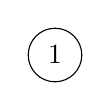
\begin{tikzpicture}\node[draw,circle,inner sep=4pt] at (0,0) {1};\end{tikzpicture}}
Soit $U$ une Algèbre \inserted{(associative avec unité) linéairement topologique, sép. et complète}
sur $\mathbb Q$, $N(U)$ l'ens de ses éléments top.
nilpotents. On définit deux \uline{bijections} \uline{réciproques}
l'une de l'autre
\diagram{\begin{tikzcd}[ampersand replacement=\&]
N(U)\arrow[r,shift left,"\exp"]\&1_U+N(U)\arrow[l,shift left,"\log"]
\end{tikzcd}}
par
\[
\left\{\begin{aligned}
\exp\deleted{\unsure{\Phi}}\inserted{\xi}&=\sum_{n\ge0}\frac1{n!}\xi^n\\
\log(1+\unsure{\eta|\zeta})&=\sum_{n>0}(-1)^{n+1}\frac1n\unsure{\eta|\zeta}^{n}
\end{aligned}\right.
\]
[N.B. Si la top. de $U$ est discrète, $N$ est l'ens. des \unsure{éléments}
nilpotents].

On a
\diagram{\begin{tikzcd}[column sep=large,ampersand replacement=\&]
\exp(\xi+\xi')=\exp\xi\exp\xi'\&\text{si }[\xi,\xi']=0\arrow[dd,Leftrightarrow]\\
\deleted{\log(1+\xi)(1+\xi')} \& \\
\log gg'=\log g\,\log g'\&\text{si }gg'=g'g
\end{tikzcd}}
\figure{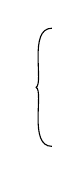
\begin{tikzpicture}\draw(.2,1.5)..controls(-.1,1.5)and(.1,.8)..(0,.75)
..controls(.1,.7)and(-.1,0)..(.2,0);\end{tikzpicture}}

Si \deleted{$\unsure{\varphi U}$} $I$ est un idéal (à gauche ou à droite)
\inserted{fermé} de $U$, on a
\diagram{\begin{tikzcd}[ampersand replacement=\&]
N(U)\cap I\arrow[r,shift left]\&1_U+N(U)\cap I\arrow[l,shift left]
\end{tikzcd}}
\margin{\deleted{$\unsure{P}$}}

Si $\varphi:U\unsure{\text{---}|\to}V$ est un hom d'anneaux \inserted{topologiques},
alors on a $\varphi(N(U))\subset N(V)$, et
\[
\left\{\begin{aligned}
\varphi\exp\xi&=\exp\varphi(\xi)\\
\varphi\log g&=\log\varphi(g)
\end{aligned}\right.
\]
\uline{Cor} \unsure{Toute|Tout} ss-algèbre fermée de $U$ est ``stable'' pour exp, log
\figure{\begin{tikzpicture}[x=1cm,y=1cm]
\draw(.3,4.6)..controls(0,4.7)and(.1,3.6)..(.1,3.4)
..controls(.1,3.2)and(0,2.7)..(.35,2.75);
\draw[->](.12,3.5)..controls(-2,1.2)and(-1.2,-1)..(1.2,-1.1);
\end{tikzpicture}}

\mspage{8}

\scanpage{10}

\figure{\begin{tikzpicture}\node[draw,ellipse,inner sep=3pt]{2};\end{tikzpicture}}
Supposons que $U$ soit \deleted{muni d'une} \inserted{une} \figure{\begin{tikzpicture}\node[draw,ellipse,inner sep=2pt] at (0,0){$k$};\node at (0,-.6){$k$};\end{tikzpicture}}-algèbre
augmentée ($k$ anneau comm.) avec un
hom diagonal
\[
\Delta:U\;\text{---}\;U\widehat\otimes_k U
\]
qui soit un hom de $k$-algèbres augmentées.
$U$ est appelée une $k$-hyperalgèbre \inserted{topologique} (au sens
large). On désigne par
\deleted{$\unsure{g(U)}$} \inserted{$\unsure{\gamma(U)|G(U)}$}
\deleted{$\unsure{G(U)}$} l'ens
des $g\in1+I(U)$ \deleted{telles que} \inserted{telles} que
\[
\Delta(g)=g\otimes g
\]
i.e.
\[
\delta\xi=\xi\otimes\xi\qquad\text{si }g=1+\xi\quad(\xi\in I(U))
\]
\margin{on suppose que $I(U)^n\longrightarrow0$ pour $n\to\infty$.
\deleted{\unsure{Donc}}}
[\deleted{éléments} ils correspondent par dualité aux
hom de la hyperalgèbre \deleted{\unsure{triviale}}
$k[T]$, avec $\delta T=T\otimes T$ ; on peut aussi
prendre $k[[T]]$, avec $\delta T=T\otimes T$, et
se borner aux hom. continus\ldots ;
cette \inserted{hyper}Algèbre est le dual top. de
l'Algèbre du groupe $\mathbb Z$ ..]. \deleted{\unsure{Ils}} Les
$g$ forment un groupe, car
\[
\Delta(gg')=\Delta(g)\Delta(g')=(g\otimes g)(g'\otimes g')
=gg'\otimes\unsure{gg'}
\]
\[
\Delta(g^{-1})=\deleted{\unsure{g\otimes}}\Delta(g)^{-1}
=(g\otimes g)^{-1}=g^{-1}\otimes g^{-1}.
\]
Fonctorialité de $\unsure{\gamma(U)|G(U)}$, et $\unsure{\pi(U)|P(U)}$
(voir ci-dessous)
\deleted{\unsure{par}} \deleted{\unsure{les}}
$(k,U)\longrightarrow(k',U')$.

\mspage{9}

\scanpage{11}

Supposons \deleted{\unsure{tjrs}} que $k$ soit une $\mathbb Q$-algèbre.
\deleted{Alors} Soit $\unsure{\pi(U)|P(U)}$
\deleted{$\unsure{\exp\xi}$} l'ens des éléments primitifs de $U$.
Alors
\deleted{\diagram{\begin{tikzcd}[ampersand replacement=\&]
\unsure{P(U)} \arrow[r] \& \unsure{G}
\end{tikzcd}}}
\diagram{\begin{tikzcd}[ampersand replacement=\&]
\pi(U) \arrow[r,bend left=15,"\exp"] \& \gamma(U) \arrow[l,bend left=15,"\log"]
\end{tikzcd}}
sont des \uline{bijections} \uline{inverses} \uline{l'une de l'autre}.

[N.B. il suffit de vérifier que exp.
applique $\pi(U)$ dans $\gamma(U)$, et log. applique
$\gamma(U)$ dans $\pi(U)$]. \uline{\unsure{Par transport de structure}},
\uline{on obtient sur} $\pi(U)$ une loi \uline{de groupe}. Elle est
donnée à l'aide du crochet, par une formule
\uline{universelle} [\unsure{formule de Campbell} \unsure{et Hausdorff}].
\margin{\uline{\unsure{f\textsuperscript{o} bell-Hausdorff}}, et coefficients des
\unsure{Séries}\unsure{---}\unsure{Exponentielle|Exponentielles}.}

\figure{\begin{tikzpicture}\node[draw,ellipse,inner sep=3pt]{3};\end{tikzpicture}}
Soit $U$ une $k$-\deleted{hyperalgèbre}
\deleted{\unsure{algèbre}} \inserted{algèbre}
\unsure{discrète} \deleted{\unsure{(i.e. séparée)}}
\deleted{\unsure{supp. que} \unsure{)}
\unsure{Alors on prend les élts|Alors on peut les exp} \unsure{)}
\unsure{et} $I(U)$ \unsure{ne soit pas nilpotent, et
exp( ) n'est pas défini a priori}}, soit
$\Lambda$ une $k$-algèbre infinitésimale.
Alors \deleted{$\unsure{K\otimes_k}$} $U\otimes_k\Lambda$ est une
$\Lambda$-hyperalgèbre augmentée ;
\deleted{\unsure{et on a là un autre} \unsure{de} l'idéal
d'augmentation $I(U)\otimes_k\Lambda$
\unsure{n'est pas nilpotent, mais on a}}
\figure{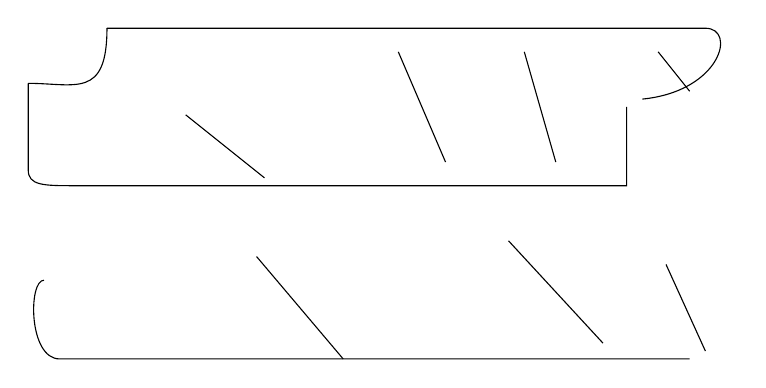
\begin{tikzpicture}[x=1cm,y=1cm]
\draw (1,4.8)--(8.6,4.8) .. controls (9,4.8) and (8.8,4) .. (7.8,3.9);
\draw (1,4.8) .. controls (1,3.9) and (.6,4.1) .. (0,4.1);
\draw (0,4.1)--(0,3) .. controls (0,2.8) and (.2,2.8) .. (.6,2.8)--(7.6,2.8)--(7.6,3.8);
\draw (2,3.7)--(3,2.9) (4.7,4.5)--(5.3,3.1) (6.3,4.5)--(6.7,3.1) (8,4.5)--(8.4,4);
\draw (.2,1.6) .. controls (0,1.6) and (0,.6) .. (.4,.6)--(8.4,.6);
\draw (2.9,1.9)--(4,.6) (6.1,2.1)--(7.3,.8) (8.1,1.8)--(8.6,.7);
\end{tikzpicture}}

\mspage{10}

\scanpage{12}

\deleted{$\unsure{I(U)}\otimes_k I(\Lambda)$ le soit.} D'où
\deleted{\diagram{\begin{tikzcd}[ampersand replacement=\&]
I(U)\otimes_k I(\Lambda) \arrow[r] \& 1+I(U)\otimes_k
\end{tikzcd}}}
\inserted{$U\otimes_k I(\Lambda)$}
\figure{\begin{tikzpicture}\draw(0,1)..controls(1.2,1)and(.1,-.2)..(1,-.2)--(2.4,-.2)..controls(2.4,.5)and(2.6,.7)..(2.9,.7);\end{tikzpicture}}

Alors $U\otimes I(\Lambda)$ est de puiss. n-ième
nulle, d'où
\diagram{\begin{tikzcd}[ampersand replacement=\&]
U\otimes I(\Lambda) \arrow[r,bend left=15,"\exp"] \& 1+U\otimes I(\Lambda) \arrow[l,bend left=15,"\log"]
\end{tikzcd}}
[et si $I(U)$ est l'idéal d'une
augmentation de $U$, on a
\diagram{\begin{tikzcd}[ampersand replacement=\&]
I(U)\otimes I(\Lambda) \arrow[r,bend left=15,"\exp"] \& 1+I(U)\otimes I(\Lambda) \arrow[l,bend left=15,"\log"]
\end{tikzcd}}]

Supposons maintenant que $U$ soit une
hyperalgèbre ordinaire. Alors la correspondance
précédente établit une corr. biunivoque
entre la partie de
\deleted{$\unsure{I(U)\otimes I(\Lambda)}$}
\inserted{$(U\otimes I(\Lambda))\cap I(U\otimes\Lambda)
\unsure{\bigl(=\Lambda\otimes_k I(U)\otimes I(\Lambda)\bigr)}$}
formée
des éléments primitifs \unsure{de} $U\otimes_k\Lambda$, et
la partie de $1+I(U)\otimes I(\Lambda)$
\deleted{$\unsure{\subset1+I(U\otimes\Lambda)}$}
formée des éléments multiplicatifs. Ce
sont aussi resp. les primitifs de
$U\otimes_k\Lambda$ qui donnent $0$ par l'augmentation
$U\otimes_k\Lambda\longrightarrow U$, et les éléments multiplicatifs de
$U\otimes_k\Lambda$ qui donnent $1$ par cette \unsure{augmentation}.

\mspage{11}

\scanpage{13}

On obtient donc des bijections inverses l'une de l'autre.
\diagram{\begin{tikzcd}[ampersand replacement=\&]
\pi_0(U\otimes\Lambda) \arrow[r,bend left=15,"\exp"] \& \gamma_0(U\otimes_k\Lambda) \arrow[l,bend left=15,"\log"]
\end{tikzcd}}
où les indices $0$ indiquent qu'on
prend les primitifs resp\textsuperscript{t} multiplicatifs
``relatifs'' à l'augmentation $U\otimes\Lambda\longrightarrow U$.

[Par passage à la limite projective \inserted{en $\Lambda$}, on déduit
un résultat analogue si $\Lambda$ est une
limite projective de $k$-algèbres infinitésimales].

Notons que \deleted{si $\Lambda$ est plat, \unsure{--- si}}
l'on a d'ailleurs un
hom canonique de $\Lambda$-modules
\diagram{\begin{tikzcd}[ampersand replacement=\&]
\pi(U)\otimes_k I(\Lambda) \arrow[r,"\alpha"] \& \pi_0(U\otimes_k\Lambda)
\end{tikzcd}}
qui est un isom si $\Lambda$ est $k$-plat,
ou si
\[
0\;\text{---}\;\deleted{\unsure{\mathfrak g}}\pi(U)
\;\text{---}\;\unsure{I(U)}\unsure{\mathrel{\overset{\delta}{\text{---}}}|\xrightarrow{\delta}}I(U)\otimes I(U)
\]
est une suite \uuline{universellement exacte}. On
en déduit donc un hom canonique
\diagram{\begin{tikzcd}[ampersand replacement=\&]
\pi(U)\otimes_k I(\Lambda) \arrow[r,"\exp\circ\alpha"] \& 1+\pi_0(U\otimes_k\Lambda)
\end{tikzcd}}
qui est un isom. dans les cas
\unsure{qu'on vient de préciser}.

\margin{[i.e. $\Delta$ est comm. et assoc,
\deleted{$\unsure{A\longrightarrow A}$}
$I(U)=\bigcup U_i$, avec $\delta U_i\subset U_i\otimes U_i$ et
$U_i$ de dim. finie, enfin $\gamma(U)=\{e\}$]}

\margin{La donnée d'une \unsure{telle} est connue quand on connaît
$\mathfrak g=\pi(U)$\deleted{$\unsure{\otimes}$}
(formule de Hausdorff-Campbell), donc
(comme par \unsure{Poincaré--B.W.} $\mathfrak g\simeq\pi(U(\mathfrak g)))$
on voit que $U\simeq U(\mathfrak g)$ avec $\mathfrak g\simeq\pi(U)$ :
\uline{th. de Cartier} $\Longleftarrow$ \unsure{précédent}.
Si $\mathfrak g$ est de dim. finie, le dual de $\unsure{\mathfrak g|U}$ est un
\uline{anneau local} \uline{régulier}. \uline{Cor} Un groupe alg. en car $0$
est \unsure{toujours lisse}.}

Conséquence : Supposons $k$ corps,
\inserted{$U$ une hyperalgèbre \uline{de Cartier}}.
Alors $U$ (avec $\Delta$ \uline{comm.} et \uline{ass.}) est connu
quand on connaît le foncteur $\pi_0(U\otimes_k\Lambda)$.

\mspage{12}

\scanpage{14}

\figure{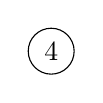
\begin{tikzpicture}\node[draw,circle,inner sep=3pt]{4};\end{tikzpicture}}
Supposons que $\unsure{U|\mathfrak g}=L_k(M)$, où $M$ est un $k$-
module, $U$ étant muni de la top. discrète.
Soit $\xi$ \uline{nilpotent} dans $U$, $g=\exp\xi$.
\[
\xi.a=0\quad\Longleftrightarrow\quad ga=a
\]
\[
\xi\text{ commute à }u\quad\Longleftrightarrow\quad g\text{ commute à }u
\]
\deleted{Supposons $\unsure{\xi}$}
\[
\begin{array}{ccc}
M'\text{ stable par }\xi&\Longleftrightarrow&M'\text{ stable par }g\\
(M'\subset M)&&
\end{array}
\]
\figure{\begin{tikzpicture}\draw[->](.3,0)..controls(-.2,0)and(0,.5)..(0,.8)--(0,1.5)--(.7,1.5);\end{tikzpicture}}

Supposons que $M$ soit muni d'une
application $k$-bilinéaire $(x,y)\longmapsto x.y$. Alors
\diagram{\[
\begin{array}{ccc}
\xi(x.y)=(\xi x)y+x(\xi y)&\Longleftrightarrow&g(x.y)=(gx)(g.y)\\
\uline{\text{dérivations}}&&\uline{\text{automorphismes}}\\
\text{nilpotentes}&&\text{unipotents}
\end{array}
\]}

\figure{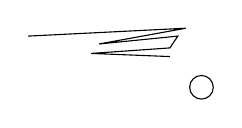
\begin{tikzpicture}\draw(0,.3)--(2,.4)--(.9,.2)--(1.9,.3)--(1.8,.15)--(.8,.08)--(1.8,.04);\draw(2.2,-.35)circle(.15);\end{tikzpicture}}

Soit $\Lambda$ une algèbre $k$-augmentée dont l'idéal
d'augmentation est \deleted{nilpotent}
\inserted{de puiss. n-ième nulle}, $k$ étant une
algèbre contenant $\mathbb Q$ \inserted{[donc $\Lambda$ contient $\mathbb Q$]},
Soit $M$ un $\Lambda$-module.
Alors les $u\in L_\Lambda(M)$ tels que $uM\subset I(\Lambda)M$
\inserted{i.e. $u$ induit $0$ dans $M\otimes_\Lambda k$}
sont nilpotents \deleted{\unsure{et les sont}}
\inserted{(de puiss. n-ième nulle)} les
$v\in L_\Lambda(M)$ tels que $v$ induise l'identité
dans $M\otimes_\Lambda k$ sont unipotents ; si \unsure{l'on}
\unsure{donne un nom à ces ensembles} $\unsure{\pi_k|\pi_\Lambda}$ resp\textsuperscript{t} $\gamma$,

\mspage{13}

\scanpage{15}

on obtient des bijections inverses l'une de l'autre
\diagram{\begin{tikzcd}[ampersand replacement=\&]
\pi \arrow[r,bend left=15,"\exp"] \& \gamma \arrow[l,bend left=15,"\log"]
\end{tikzcd}}
Bien entendu, $\pi$ est un idéal \inserted{(nilpotent)} de $L_\Lambda(M)$, et
à fortiori une sous-algèbre de Lie. En
transportant à $\pi$ la structure de groupe de
$\gamma$, on trouve une structure de groupe \unsure{dans}
$\pi$, qui se déduit de sa structure
d'algèbre de Lie par la formule de
Hausdorff-Campbell. Si $M$ est une
$\Lambda$-Algèbre \inserted{$\unsure{B|A}$}, on trouve le

\uline{Corollaire} les \uline{automorphismes} de la
$\Lambda$-algèbre \uline{$\unsure{B|A}$} (où $\Lambda$ est une algèbre
$k$-augmentée : \deleted{\unsure{ayant}} idéal d'augmentation
nilpotent, $k$ est une $\mathbb Q$-algèbre)
qui induisent l'identité sur $B\otimes_\Lambda k$
correspondent biunivoquement aux
$\Lambda$-dérivations \inserted{$D$} de $B$ telles que $DB\subset I(\Lambda)B$.

\mspage{14}

\scanpage{16}

Supposons en particulier
\[
B=A\otimes_k\Lambda
\]
où $\Lambda$ est une $k$-algèbre infinitésimale.
Alors \deleted{$\unsure{\Omega^1_\Lambda}$}
\[
\begin{aligned}
\mathfrak g_{B/\Lambda}\deleted{\unsure{(\Omega_\Lambda)}}
&=\operatorname{Hom}_B(\Omega^{\unsure{1|'}}_{B/\Lambda},B)
\simeq\operatorname{Hom}_B(\Omega^{\unsure{1|'}}_{A/k}\otimes_k\Lambda,A\otimes_k\Lambda)\\
&\simeq\operatorname{Hom}_A(\Omega^{\unsure{1|'}}_{A/k},A\otimes_k\Lambda)
\simeq\text{$k$-dérivations}\\
&\hspace{7cm}\text{de $A$ dans $A\otimes_k\Lambda$}
\end{aligned}
\]
et les $\Lambda$-dérivations de $B$ dans $B$ qui
induisent $0$ sur $B\otimes_\Lambda k\simeq\unsure{\Lambda|A}$ s'identifient
aux $k$-dérivations $A\;\text{---}\;A\otimes_k I(\Lambda)$.
Donc

\uline{Proposition} Supposons $k$ \deleted{\unsure{de}} $\supset\mathbb Q$, $A$ une
$k$-alg. comm., $\Lambda$ une $k$-alg. inf.
Alors \unsure{le|les} \inserted{groupe de} $\Lambda$-autom. infinitésimaux de
$A\otimes_k\Lambda$ \deleted{\unsure{sont en co}} est isomorphe
à l'ens des $k$-dérivations de
$A$ dans $A\otimes_k I(\Lambda)$, avec la structure
de groupe donnée par Hausdorff-
Campbell.
\figure{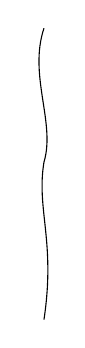
\begin{tikzpicture}\draw(0,0)..controls(.15,1)and(-.1,1.4)..(0,2)..controls(.15,2.5)and(-.2,3.1)..(0,3.7);\end{tikzpicture}}

\mspage{15}
